% !TEX TS-program = pdflatex
% !TEX root = manuscript-2.tex
% !TEX TS-use-input-relative-path = true
% IEEE TWC: abstract 75--200 words; manuscript $\leq$13 pages (first submission);
% scope requires a wireless communications problem with channel effects (e.g., fading/coupling) central.
\documentclass[journal]{IEEEtran}
\usepackage{amsmath,amsfonts,amssymb}
\usepackage[ruled,vlined]{algorithm2e}
\usepackage{array}
\usepackage[caption=false,font=normalsize,labelfont=sf,textfont=sf]{subfig}
\usepackage{textcomp}
\usepackage{url}
\usepackage{verbatim}
\usepackage{graphicx}
\usepackage{dblfloatfix}
\usepackage{cite}
\usepackage{makecell}
\usepackage{multirow}
\usepackage{tabularx}
\usepackage{booktabs}
\usepackage{tikz}
\usetikzlibrary{arrows.meta,positioning,shapes.geometric}
\usepackage{hyperref}
\hypersetup{hidelinks}
\usepackage{orcidlink}
\hyphenation{op-tical net-works semi-conduc-tor IEEE-Xplore}
\DontPrintSemicolon
\SetKwInput{KwInput}{Input}
\SetKwInput{KwOutput}{Output}
% Encourage floats to stay near callouts in IEEE two-column layout.
\setcounter{topnumber}{2}
\setcounter{dbltopnumber}{2}
\renewcommand{\topfraction}{0.9}
\renewcommand{\dbltopfraction}{0.9}
\renewcommand{\textfraction}{0.07}
\renewcommand{\floatpagefraction}{0.8}
\renewcommand{\dblfloatpagefraction}{0.8}
% Float sizing: single-column figures use \linewidth; double-column use \textwidth.
% Fig.~2 and Fig.~3 (vertical flowcharts): inset within the column so left/right margins remain visible.
\newcommand{\figcol}{\linewidth}
\newcommand{\figcolvertw}{0.86\linewidth}
\newcommand{\figcolverth}{0.56\textheight}
% Double-column (\texttt{figure*}) widths: tune per figure.
\newcommand{\figdbl}{0.98\textwidth}% default wide star figures (e.g., merged BER)
\newcommand{\figdblone}{0.6\textwidth}% Fig.~1: comprehensive system model
\newcommand{\figdblfour}{0.51\textwidth}% Fig.~4: neural inference (0.66 - 0.15)
\newcommand{\figdblfive}{0.66\textwidth}% Fig.~5: curriculum (0.76 - 0.10)
\newcommand{\figdblnine}{0.68\textwidth}% Fig.~9: merged BER (0.98 - 0.30)
% Uniform subfigure layout for Fig.~8 and Fig.~10.
\newcommand{\subfigw}{0.31\textwidth}
\newcommand{\subfiggap}{2pt}

\begin{document}

\title{OAM-Assisted High-Capacity Transmission: A Link-Level Performance Study}

\author{Srivatsa~Davuluri\textsuperscript{\orcidlink{0000-0000-0000-0000}},
        Baskar~P\textsuperscript{\orcidlink{0000-0000-0000-0000}},
        Abhijit~Bhowmick\textsuperscript{\orcidlink{0000-0000-0000-0000}},
        Sudhanshu~Arya\textsuperscript{\orcidlink{0000-0000-0000-0000}}%

}

\maketitle
\markboth{IEEE Transactions on Wireless Communications}{Davuluri \MakeLowercase{\textit{et al.}}: Baseline-Validated OAM Receiver Under Turbulence}


\begin{abstract}
Optical wireless links using orbital angular momentum (OAM) spatial multiplexing promise high spectral efficiency, but atmospheric turbulence induces fading-like scintillation and random mode coupling that acts as structured spatial interference among parallel streams. Fair evaluation of machine-learning receivers therefore requires a classical baseline under identical channel statistics. We develop an end-to-end framework: LDPC-coded quadrature phase-shift keying (QPSK) on eight Laguerre--Gaussian modes, split-step Fourier propagation with Kolmogorov phase screens, aperture observation, coherent modal projection, pilot-aided least-squares estimation, minimum mean-square error (MMSE) equalization, blind phase recovery, and LDPC decoding. Across a sweep of the refractive-index structure parameter $C_n^2$, we report modal overlap, pre- and post-decoding bit-error rate (BER), the condition number $\kappa(\hat{\mathbf{H}})$, and $|\hat{\mathbf{H}}|$. The coherent receiver is near error-free for $C_n^2 \lesssim 10^{-16}$, then degrades as $\kappa(\hat{\mathbf{H}})$ grows toward $\sim 17$ and forward-error-correction gain vanishes near $C_n^2 \approx 10^{-14}$. An intensity-only convolutional receiver (ConvNeXt, polar loss, five-stage curriculum) trained on matched data retains useful BER in weak-to-moderate turbulence but approaches random guessing under strong and extreme conditions, exposing limits of pilot-free phase-blind recovery relative to coherent processing.
\end{abstract}

\begin{IEEEkeywords}
Wireless optical communications, free-space optics, orbital angular momentum, spatial multiplexing, atmospheric turbulence, channel estimation, LDPC codes, deep learning, convolutional neural networks.
\end{IEEEkeywords}

%==============================================================================
% I. INTRODUCTION
%==============================================================================
\section{Introduction}
\label{sec:intro}

\IEEEPARstart{W}{ireless} communication increasingly relies on spatial degrees of freedom---from multiple antennas in radio to mode-division multiplexing in optical fibers and \emph{optical wireless} links---to raise throughput without proportional bandwidth growth. Free-space optical transmission addresses short- and medium-range connectivity---campus interconnects, temporary backhaul, airborne relays, and scenarios where fiber is costly or impossible---using narrow beams, license-free spectrum, and mature photonics~\cite{khalighi2014survey, kaushal2016optical}. Orbital angular momentum (OAM) multiplexing is one such spatial approach: distinct Laguerre--Gaussian (LG) modes carry parallel streams when orthogonality is preserved end-to-end~\cite{allen1992orbital, wang2012terabit, willner2015optical}. The effective spatial channel is then analogous to a multi-input multi-output (MIMO) mixing matrix in the mode domain; the design question is how that matrix behaves once the outdoor channel is random rather than ideal.

The limiting factor in outdoor optical wireless links is the atmosphere. Turbulent eddies impose random phase and amplitude distortions along the path, producing scintillation (fading-like intensity fluctuations), beam wander, and inter-modal coupling~\cite{andrews2005laser, paterson2005atmospheric, ren2013atmospheric}. For OAM systems, the practical effect is loss of spatial orthogonality: energy leaks across modes, the mode-domain channel matrix $\mathbf{H}$ becomes dense and ill-conditioned, and coherent receivers must equalize before soft information can be passed to an FEC decoder---precisely the setting in which wireless receiver design is traditionally analyzed.

Classical digital signal processing for OAM links---coherent projection onto a mode basis, pilot-aided channel estimation, linear or near-optimal equalization, and forward error correction---remains the interpretable benchmark against which new algorithms should be judged~\cite{huang2014100, ge2021oam}. When turbulence is mild, these chains perform well; when coupling strengthens, equalization amplifies noise and soft likelihood ratios delivered to the LDPC decoder collapse, eroding coding gain. Machine learning is a natural complement because it can map high-dimensional observations to symbols without explicit matrix inversion, yet published OAM studies often emphasize mode classification, compensation submodules, or unequal simulation assumptions~\cite{liu2019oam_prl, doster2017machine, karanov2018endtoend, zhao2020cnn, lohani2018turbulence, arya2023oam}. In the studies reviewed here, two gaps stand out: (i)~few works couple a turbulence-aware physical simulator to a full LDPC-inclusive classical receiver evaluated on identical data and turbulence settings, and (ii)~intensity-only neural receivers are rarely compared under the same $C_n^2$ sweep as a validated coherent baseline.

This paper narrows those gaps with a baseline-first methodology. We construct a single end-to-end pipeline---multiplexed QPSK on eight OAM modes, split-step Fourier propagation with Kolmogorov screens, aperture observation, pilot-aided least-squares estimation, MMSE equalization, phase recovery, and LDPC decoding---and sweep $C_n^2$ systematically to map where BER remains low, where the estimated channel matrix becomes ill-conditioned, and where FEC gain disappears. We then instantiate an intensity-only convolutional neural receiver trained with a five-stage curriculum on physics-generated intensity images drawn from the same simulator, enabling a controlled comparison under matched channels at 1550~nm over 1~km. The classical receiver is near error-free up to about $C_n^2 \approx 10^{-16}$, transitions as $\kappa(\hat{\mathbf{H}})$ rises, and saturates near BER $0.5$ beyond $\sim 10^{-14}$; the neural receiver remains useful in weak-to-moderate regimes but loses reliability under the strongest distortions, consistent with phase-sensitive turbulence effects reported in prior OAM studies~\cite{ren2013atmospheric, paterson2005atmospheric}.

The primary contributions of this paper are as follows:
\begin{itemize}
\item End-to-end turbulence-aware receiver framework for OAM-multiplexed optical links, covering beam generation, turbulent propagation, coherent modal projection, pilot-aided channel estimation, MMSE equalization, and LDPC decoding in a single physically grounded simulation.

\item Validated classical baseline across turbulence regimes, characterized by BER curves, pre-/post-decoding comparisons, and channel-matrix visualizations, showing where modal coupling sets in and where decoding gain becomes unreliable.

\item Consistent neural-receiver framework and training protocol, formulated as an intensity-only curriculum-based extension of the same physical pipeline, so that future comparisons are against a verified reference rather than an uncalibrated one.
\end{itemize}

A few sub-problems in the existing literature bear directly on what is done here. Turbulence propagation for OAM links is typically modeled via split-step Fourier methods~\cite{schmidt2010numerical} and Kolmogorov phase screens~\cite{andrews2005laser}; LDPC coding is widely used for FEC in optical systems~\cite{richardson2008modern}. Classical DSP approaches for OAM demultiplexing include MMSE equalization~\cite{huang2014100} and K-best detection~\cite{ge2021oam}. Existing deep-learning studies have generally focused on mode classification or turbulence-compensation subproblems rather than end-to-end symbol recovery~\cite{liu2019oam_prl, doster2017machine, karanov2018endtoend, zhao2020cnn}. OAM mode classification and demultiplexing using CNNs have been explored by several groups~\cite{lohani2018turbulence, doster2017machine, arya2023oam}; others have applied deep learning to optical signal detection and turbulence compensation tasks~\cite{karanov2018endtoend, zhao2020cnn}. Table~\ref{tab:comparison} places the present work alongside these studies.

The paper is organized as follows. Section~\ref{sec:channel} develops the link model and describes the classical MMSE+LDPC baseline. Section~\ref{sec:neural} covers the neural receiver architecture and curriculum training. Results are presented and interpreted in Section~\ref{sec:results}. Section~\ref{sec:conclusion} concludes.

\begin{table*}[!t]
\centering
\caption{Comparison with Related Work}
\label{tab:comparison}
\footnotesize
\setlength{\tabcolsep}{5pt}
\renewcommand{\arraystretch}{1.1}
\begin{tabular}{lcccccc}
\toprule
\textbf{Method} & \makecell{\textbf{Symbol}\\\textbf{Recovery}} & \textbf{Coherent} & \makecell{\textbf{Pilot}\\\textbf{Aided}} & \makecell{\textbf{Optical}\\\textbf{Wireless/OAM}\\\textbf{Turbulence}} & \makecell{\textbf{End-to-}\\\textbf{End}} & \makecell{\textbf{Weak}\\\textbf{$\rightarrow$ Extreme Sweep}} \\
\midrule
MMSE~\cite{huang2014100} & \checkmark & \checkmark & \checkmark & \checkmark & -- & -- \\
K-best~\cite{ge2021oam} & \checkmark & \checkmark & \checkmark & \checkmark & -- & -- \\
CNN (Mode)~\cite{doster2017machine} & -- & -- & -- & \checkmark & -- & -- \\
End-to-end DL~\cite{karanov2018endtoend} & \checkmark & -- & -- & -- & \checkmark & -- \\
AlexNet~\cite{zhao2020cnn} & -- & -- & -- & \checkmark & -- & -- \\
\midrule
\textbf{This work} & \checkmark & \checkmark & \checkmark & \checkmark & \checkmark & \checkmark \\
\bottomrule
\end{tabular}
\vspace{0.7mm}
\parbox{0.95\textwidth}{\footnotesize\textit{Legend:} ``Symbol Recovery'' denotes direct symbol recovery output. ``Coherent'' denotes coherent modal observation. ``Optical Wireless/OAM Turbulence'' denotes modeling/evaluation on free-space OAM turbulence channels.}
\end{table*}

%==============================================================================
% II. CHANNEL MODEL AND CLASSICAL RECEIVER BASELINE [Methods]
%==============================================================================
\section{Channel Model and Classical Receiver Baseline}
\label{sec:channel}

Acronyms are listed in Table~\ref{tab:abbreviations}. What follows develops the OAM optical link model and the classical receiver built on top of it. The shared front end maps coded QPSK symbols onto multiplexed LG modes, propagates through Kolmogorov turbulence with a swept $C_n^2$, and forms observations for coherent processing and neural evaluation under matched channel assumptions.

\begin{table}[htbp]
\centering
\caption{Abbreviations and Acronyms}
\label{tab:abbreviations}
\small
\renewcommand{\arraystretch}{1.1}
\begin{tabular}{ll}
\toprule
\textbf{Acronym} & \textbf{Definition} \\
\midrule
AWGN & Additive White Gaussian Noise \\
BER & Bit Error Rate \\
$C_n^2$ & Refractive-index structure parameter (m$^{-2/3}$) \\
LG & Laguerre-Gaussian \\
LDPC & Low-Density Parity-Check \\
LS & Least Squares \\
MMSE & Minimum Mean-Square Error \\
OAM & Orbital Angular Momentum \\
QPSK & Quadrature Phase Shift Keying \\
SNR & Signal-to-Noise Ratio \\
SSFM & Split-Step Fourier Method \\
\bottomrule
\end{tabular}
\end{table}


The link model rests on superimposed Laguerre-Gaussian (LG) beams propagated through the turbulence channel using split-step Fourier simulation. At the transmitter, independent coded data streams are modulated to QPSK symbols $s_m \in \{ \pm \frac{1}{\sqrt{2}} \pm j\frac{1}{\sqrt{2}} \}$, one per spatial mode $m \in \{1, 2, \dots, M\}$, and each symbol then modulates the corresponding orthogonal LG beam. The complex electric field of an LG beam with radial index $p$ and azimuthal index (topological charge) $l$, at the beam waist ($z=0$), is described as
\begin{equation}
\label{eq:lg_beam}
\begin{split}
    E_{p,l}(r, \phi, 0) &= \sqrt{\frac{2 p!}{\pi (p + |l|)!}} \frac{1}{w_0} \left( \frac{\sqrt{2} r}{w_0} \right)^{|l|} \\
    &\quad \times L_p^{|l|}\left( \frac{2 r^2}{w_0^2} \right) \exp\left( -\frac{r^2}{w_0^2} \right) \exp(-j l \phi),
\end{split}
\end{equation}
where $(r, \phi)$ are polar coordinates, $w_0$ is the beam waist, and $L_p^{|l|}(\cdot)$ is the generalized Laguerre polynomial~\cite{allen1992orbital}. For this study, $p=0$ to minimize beam divergence. The total transmitted field is defined as
\begin{equation}
\label{eq:tx_field}
    E_{\mathrm{tx}}(r, \phi, 0) = \sum_{m=1}^{M} s_m E_{0, l_m}(r, \phi, 0).
\end{equation}

Propagation is modeled using the split-step Fourier method (SSFM)~\cite{schmidt2010numerical} with phase screens drawn from the Kolmogorov spectrum~\cite{andrews2005laser, tatarskii1971wave}. The refractive-index power spectral density is described as
\begin{equation}
\label{eq:kolmogorov}
    \Phi_{n}(\kappa_{\mathrm{sf}}) = 0.033\, C_n^2\, \kappa_{\mathrm{sf}}^{-11/3},
\end{equation}
where $C_n^2$ (in m$^{-2/3}$) is the refractive-index structure parameter and $\kappa_{\mathrm{sf}}$ is the spatial angular frequency (rad/m), distinct from the matrix condition number $\kappa(\hat{\mathbf{H}})$ used later. At lower turbulence levels ($C_n^2 \approx 10^{-16}$), the beam arrives largely intact; once $C_n^2$ climbs to $10^{-14}$ or above, phase-front distortions are severe. After propagation, each coherent projection of $E_{\mathrm{rx}}(r, \phi, Z)$ onto the reference LG set generally depends on several transmitted symbols, not only the symbol on mode $m$; modal orthogonality is therefore lost in the sense that the effective mapping from $\mathbf{s}$ to the projected vector $\mathbf{y}$ is a full $M \times M$ mixing channel, modeled next as $\mathbf{y} = \mathbf{H}\mathbf{s} + \mathbf{n}$.

Table~\ref{tab:link_params} lists the link and simulation parameters. Attenuation includes free-space path loss and geometric loss; the receiver aperture clips the field before coherent projection. Modal overlap versus $C_n^2$ is analyzed later in Section~\ref{sec:results} alongside BER and channel-matrix results.

\begin{figure*}[!t]
\centering
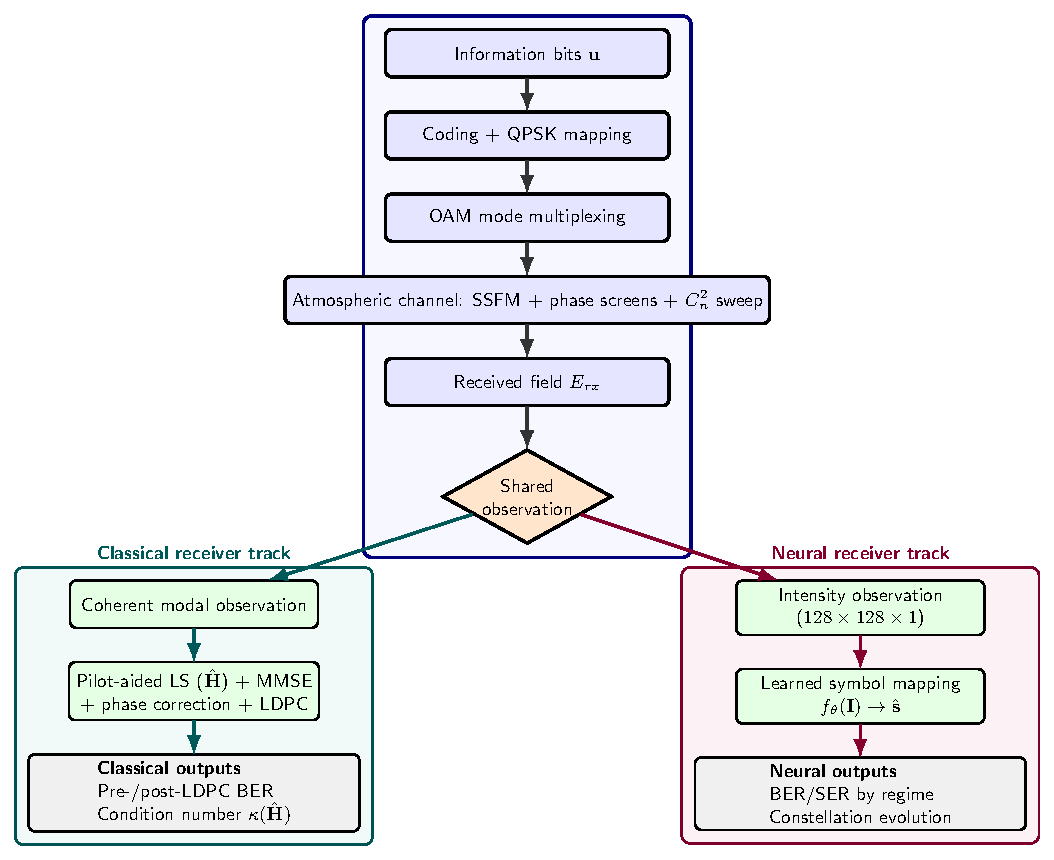
\includegraphics[width=\figdblone]{images/system_model_diagram.pdf}
\caption{Comprehensive OAM optical system model with a shared propagation backbone and two receiver tracks. The shared chain maps coded QPSK symbols onto multiplexed OAM modes, propagates through turbulence ($C_n^2$ sweep), and forms a common received observation. The classical branch performs coherent observation and pilot-aided LS/MMSE recovery, while the neural branch performs intensity-based learned symbol mapping; both are evaluated under matched channel assumptions.}
\label{fig:comprehensive_system_model}
\end{figure*}

\begin{figure}[htbp]
\centering
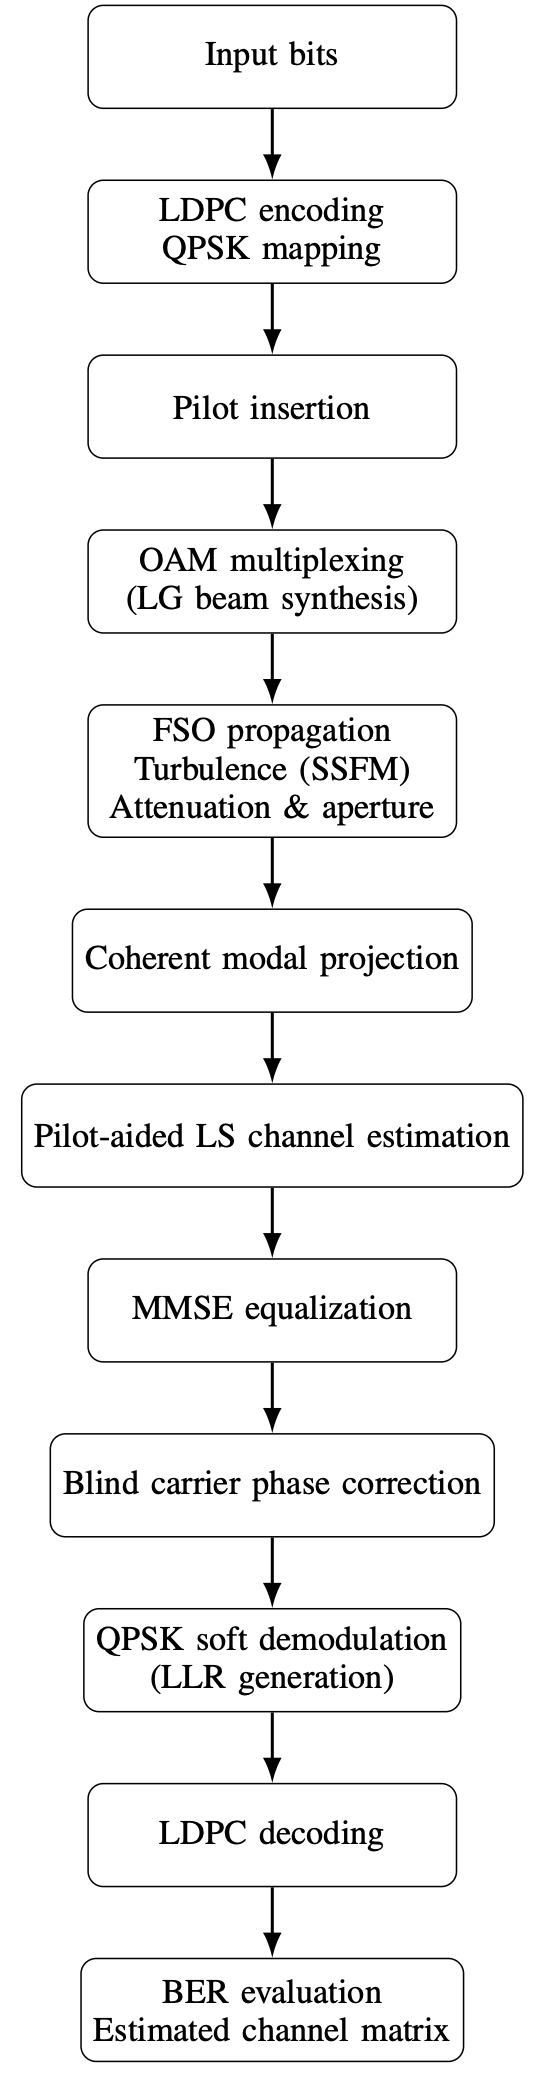
\includegraphics[width=\figcolvertw,height=\figcolverth,keepaspectratio]{images/classical/system_architecture.png}
\caption{Classical baseline receiver architecture for OAM-multiplexed optical links. Data flows from encoding and modulation through turbulent propagation to coherent modal projection, pilot-aided channel estimation, MMSE equalization, blind carrier phase correction, and LDPC decoding.}
\label{fig:system_architecture}
\end{figure}

\begin{table}[htbp]
\centering
\caption{Link and Simulation Parameters}
\label{tab:link_params}
\small
\renewcommand{\arraystretch}{1.1}
\begin{tabular}{l l}
\toprule
\textbf{Parameter} & \textbf{Value} \\
\midrule
Wavelength $\lambda$ & 1550~nm \\
Link distance $L$ & 1~km \\
Beam waist $w_0$ & 25~mm \\
Receiver aperture & 500~mm diameter \\
Spatial modes $M$ & 8: $(0,\pm1)$, $(0,\pm3)$, $(0,\pm4)$, $(1,\pm1)$ \\
Modulation & QPSK \\
LDPC rate & 0.8 ($n=2048$, $k \approx 1638$) \\
Pilot ratio & 10\% (preamble + comb) \\
SSFM grid & $512 \times 512$ \\
Phase screens & 25 (uniform $C_n^2$ profile) \\
SNR (at receiver) & 35~dB \\
\bottomrule
\end{tabular}
\end{table}


The classical receiver has coherent access to the modal projections and a set of known pilot symbols, which allows the channel to be estimated and MMSE equalization applied before passing soft information to the LDPC decoder. The analog field is first demultiplexed via coherent matched filtering. The $m$th projected output is defined as
\begin{equation}
\label{eq:mode_projection}
    y_m = \iint E_{\mathrm{rx}}(r, \phi, Z)\, E_{0, l_m}^{*}(r, \phi, Z)\, r \,\mathrm{d}r \,\mathrm{d}\phi.
\end{equation}
The received symbol vector $\mathbf{y} \in \mathbb{C}^{M}$ is related to the transmitted vector $\mathbf{s} \in \mathbb{C}^{M}$ by the linear model
\begin{equation}
\label{eq:linear_channel}
    \mathbf{y} = \mathbf{H} \mathbf{s} + \mathbf{n},
\end{equation}
where $\mathbf{H} \in \mathbb{C}^{M \times M}$ is the crosstalk channel matrix and $\mathbf{n}$ denotes circular AWGN with variance $\sigma^2$. The condition number $\kappa(\hat{\mathbf{H}}) = \|\hat{\mathbf{H}}\|_2 \,\|\hat{\mathbf{H}}^{-1}\|_2$ (for invertible $\hat{\mathbf{H}}$) summarizes numerical sensitivity of inversion and equalization; large $\kappa(\hat{\mathbf{H}})$ indicates that small perturbations or noise are amplified at the output of $\mathbf{W}_{\mathrm{MMSE}}$. Using interleaved pilots, the receiver estimates $\hat{\mathbf{H}}$ via least-squares estimation~\cite{kay1993fundamentals}. The MMSE equalization weight matrix is defined as~\cite{kay1993fundamentals}
\begin{equation}
\label{eq:mmse}
    \mathbf{W}_{\mathrm{MMSE}} = \hat{\mathbf{H}}^{\mathrm{H}} \left( \hat{\mathbf{H}} \hat{\mathbf{H}}^{\mathrm{H}} + \frac{\sigma^2}{\sigma_s^2} \mathbf{I} \right)^{-1},
\end{equation}
where $(\cdot)^{\mathrm{H}}$ is the Hermitian transpose, $\sigma_s^2$ is the nominal symbol power, and $\mathbf{I}$ is the $M \times M$ identity matrix. Equalized symbols are converted to soft log-likelihood ratios (LLRs) and passed to the LDPC decoder, yielding both pre- and post-decoding BER. Residual carrier phase is corrected with a blind fourth-power estimator~\cite{viterbi1983nonlinear}. Under strong turbulence, $\mathbf{H}$ becomes ill-conditioned and the inversion in (\ref{eq:mmse}) grows unstable, at which point the coding gain that LDPC provides essentially vanishes. Algorithms~\ref{alg:tx_pipeline} and~\ref{alg:baseline_receiver} provide pseudocode for the transmitter and receiver pipelines.

\begin{algorithm}[t]
\caption{OAM Transmitter Pipeline}
\label{alg:tx_pipeline}
\KwInput{Info bits $\mathbf{u}$, $M$ spatial modes, LDPC rate, pilot ratio $\rho$}
\KwOutput{Received field sequence $\{E_{rx}^{(\tau)}\}$, tx signals, grid info}
Encode $\mathbf{u}$ with LDPC, modulate to QPSK symbols, and partition across $M$ modes\;
Insert pilots (preamble + comb) per mode and record pilot positions\;
\For{each symbol slot $\tau$}{
Form multiplexed field: $E_{tx} \leftarrow \sum_m s_m \cdot E_{0,l_m}$ (scaled LG basis)\;
Propagate: $E_{rx} \leftarrow \mathrm{SSFM}(E_{tx})$; apply attenuation and AWGN; clip to aperture\;
}
\Return{Received field sequence $\{E_{rx}^{(\tau)}\}$, tx signals, grid info}
\end{algorithm}

In words, the transmitter pipeline repeatedly encodes information bits with the LDPC code, maps them to QPSK symbols, inserts known pilots for channel estimation, forms the multiplexed LG field for each symbol interval, and propagates that field through the SSFM turbulence simulator with attenuation and noise before returning the sequence of received fields needed by either receiver branch.

\begin{algorithm}[t]
\caption{Classical MMSE+LDPC Receiver}
\label{alg:baseline_receiver}
\KwInput{Received fields $\{E_{rx}^{(\tau)}\}$, tx signals, ground-truth bits $\mathbf{u}$}
\KwOutput{Decoded bits $\hat{\mathbf{u}}$, BER (pre/post LDPC), estimated channel $\hat{\mathbf{H}}$}
Project each field onto the LG basis: $y_m = \langle E_{rx}, E_{ref,m} \rangle$ (coherent matched filter)\;
Estimate channel $\hat{\mathbf{H}}$ from pilots via least squares and estimate noise $\sigma^2$ from pilot residuals\;
Extract data symbols $\mathbf{Y}_d$ and exclude pilot positions\;
Compute MMSE weights $\mathbf{W} = \hat{\mathbf{H}}^H (\hat{\mathbf{H}}\hat{\mathbf{H}}^H + \frac{\sigma^2}{\sigma_s^2}\mathbf{I})^{-1}$; equalize: $\hat{\mathbf{S}} = \mathbf{W}\mathbf{Y}_d$\;
Apply blind phase correction (4th-power method) and normalize\;
Demodulate to soft LLRs and compute pre-LDPC BER\;
Decode LLRs with LDPC belief propagation, extract info bits $\hat{\mathbf{u}}$, and compute post-LDPC BER\;
\Return{$\hat{\mathbf{u}}$, BER, $\hat{\mathbf{H}}$}
\end{algorithm}

The classical receiver therefore mirrors standard practice: it projects each snapshot onto the reference LG modes, estimates the mixing matrix and noise level from pilots, applies MMSE weights to data symbols, removes residual carrier phase, forms soft bits, and finally runs belief propagation on the LDPC graph so that both uncoded and coded error rates can be reported alongside $\hat{\mathbf{H}}$ for visualization.

Taken together, the shift from near-diagonal to diffuse channel structure as $\kappa(\hat{\mathbf{H}})$ rises from about 1 toward 17 marks the region where classical inversion starts to fail and where a data-driven approach might help.

%==============================================================================
% III. NEURAL RECEIVER FRAMEWORK [Methods]
%==============================================================================
\section{Neural Receiver Framework}
\label{sec:neural}

The classical chain in Section~\ref{sec:channel} becomes ill-conditioned when turbulence-induced coupling strengthens, so that MMSE equalization and FEC face the same noise-amplification limits summarized by rising $\kappa(\hat{\mathbf{H}})$. A learned receiver offers an alternative mapping from observations to symbols without explicit pilot-based matrix inversion; here we restrict observations to intensity-only images so that the comparison isolates what can be recovered without phase references or coherent projection. The neural receiver is trained on data from the same SSFM backbone as the baseline. Fig.~\ref{fig:neural_vs_classical} shows the two branches side by side.

\begin{figure}[htbp]
\centering

\includegraphics[width=0.45\linewidth]{images/neural/system_architecture.png}
\caption{High-level comparison: classical branch uses coherent projection and pilot-aided MMSE; neural branch uses intensity-only input and learned mapping $f_\theta$. Both share the same optical propagation model.}
\label{fig:neural_vs_classical}
\end{figure}


The neural receiver takes raw intensity images as input and tries to recover the transmitted symbols directly, without any coherent projection or channel estimation step. Intensity images discard the phase of the received field entirely, which is a significant information loss relative to coherent detection; the trade-off is that no phase reference or pilot overhead is needed. The \texttt{OpticalWirelessModel} accepts a single-channel, normalized intensity image $\mathbf{I} \in \mathbb{R}^{H \times W \times 1}$ ($H=W=128$) and outputs $M$ complex QPSK symbols. The input--output map is described as
\begin{equation}
\label{eq:fso_model}
    \hat{\mathbf{s}} = f_{\theta}(\mathbf{I}),
\end{equation}
where $f_{\theta}$ denotes the trainable network with parameters $\theta$. In place of coherent projection, channel estimation, and MMSE equalization, everything is folded into a single learned function of the intensity image. The backbone is either ConvNeXt~\cite{liu2022convnet} or EfficientNet~\cite{tan2019efficientnet}, with the stem modified for single-channel optical input by averaging the pre-trained RGB weights across channels (``Smart Initialization''), which lets the model start from a reasonable feature set without retraining the backbone from scratch. The projection head regresses latent features down to $2M$ real values for the I/Q components. Fig.~\ref{fig:neural_inference} shows the inference path from optical propagation through intensity capture to symbol regression and BER evaluation at coded level.

\begin{figure*}[!t]
\centering
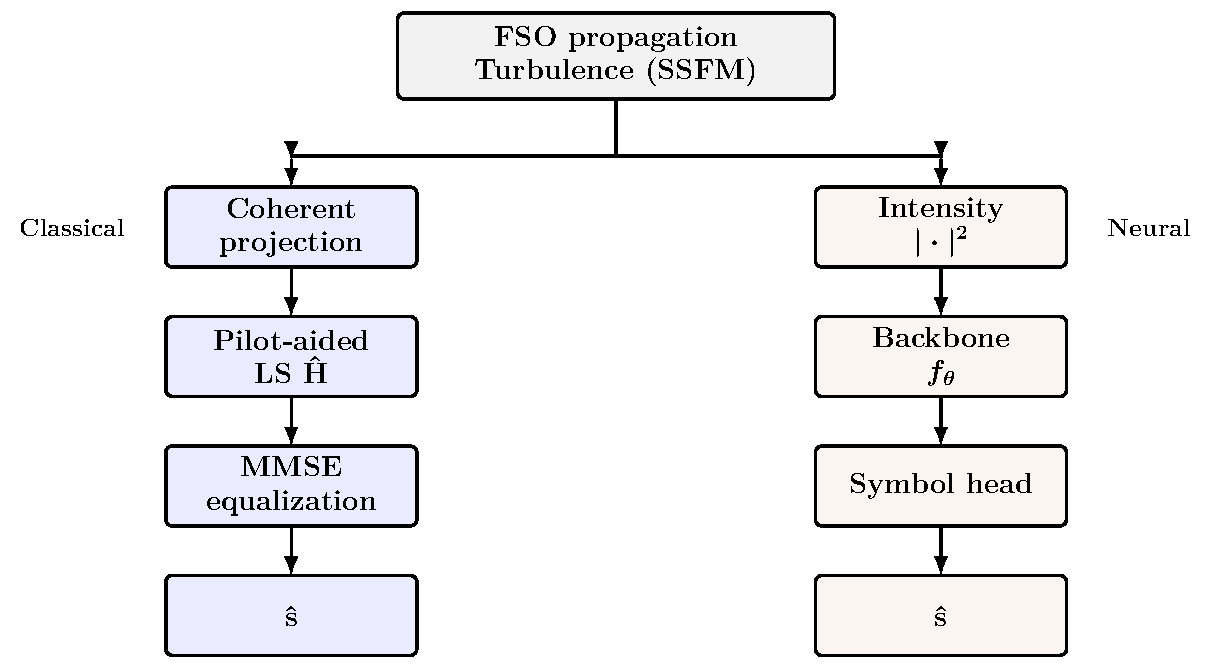
\includegraphics[width=\figdblfour]{images/neural/fso_turbulence_prop.pdf}
\caption{Neural receiver inference architecture. Intensity-only input flows through stem adaptation, backbone, and a projection head that regresses $M$ complex QPSK symbols. BER/SER is evaluated at coded level (QPSK demodulation to bits). No LDPC decoding stage is used here, allowing direct comparison with the classical chain at pre-LDPC level.}
\label{fig:neural_inference}
\end{figure*}


% \FloatBarrier
Training pairs a physics-generated dataset with a five-stage curriculum, chiefly to sidestep the gradient collapse that direct training on extreme turbulence tends to cause. The training data consists of physics-generated HDF5 datasets: each sample is a single-channel $128 \times 128$ intensity map paired with an $8 \times 2$ real tensor holding the I/Q components of the eight transmitted QPSK symbols. Each stage draws 50{,}000 training samples, 5{,}000 for validation, and 5{,}000 for test, with $C_n^2$ drawn on a log scale across the stage's range. The five stages cover ideal/very weak ($10^{-18}$--$10^{-17}$), weak ($10^{-17}$--$10^{-16}$), moderate ($10^{-16}$--$10^{-15}$), strong ($10^{-15}$--$10^{-14}$), and extreme ($10^{-14}$--$10^{-12}$) turbulence. Inputs are stored with per-sample normalization; standard ImageNet-style channel renormalization is intentionally skipped so the network processes physics-scaled intensity values as-is.

Plain mean-squared error (MSE) is a poor fit for QPSK regression because it is indifferent to phase errors between predicted and true symbols. We instead use a phase-aware polar loss, defined as
\begin{equation}
\label{eq:polar_loss}
    \mathcal{L}_{\mathrm{Polar}} = \alpha\, \mathrm{MSE}\bigl(|\mathbf{s}|, |\hat{\mathbf{s}}|\bigr) + \beta\, \bigl(1 - \cos(\angle \mathbf{s} - \angle \hat{\mathbf{s}})\bigr),
\end{equation}
which penalizes magnitude and phase errors separately. In practice, $\alpha=\beta=1.0$ worked well; adjusting these weights is left as a tuning option.

The data loader also supports optional physics-aware rotations by integer multiples of $90^\circ$, together with the corresponding OAM-consistent symbol update, described as
\begin{equation}
\label{eq:rotation_aug}
    \tilde{s}_m = s_m \exp(-j l_m \alpha), \qquad \alpha \in \left\{0,\, \frac{\pi}{2},\, \pi,\, \frac{3\pi}{2}\right\},
\end{equation}
where $l_m$ is the azimuthal index of the $m$th mode. Rotated intensity images with their adjusted labels are thus physically consistent with the original data. For the curriculum runs reported here, augmentation was left off across all five stages because the goal was to isolate the curriculum effect. It remains available for follow-on experiments.

Training directly on extreme turbulence ($C_n^2 \ge 10^{-13}$) causes gradient collapse. Instead, we follow a physics-aware curriculum~\cite{bengio2009curriculum, soviany2022curriculum} that mirrors the physical ordering of regimes: stage~1 (ideal/very weak), then stage~2 (weak), stage~3 (moderate), stage~4 (strong), and stage~5 (extreme), with $C_n^2$ drawn log-uniformly within the bands stated at the start of this section. The best checkpoint from each stage initializes the next, so optimization accumulates rather than restarting from scratch on harsh statistics alone. Fig.~\ref{fig:neural_curriculum} illustrates the training pipeline.

\begin{figure*}[!t]
\centering
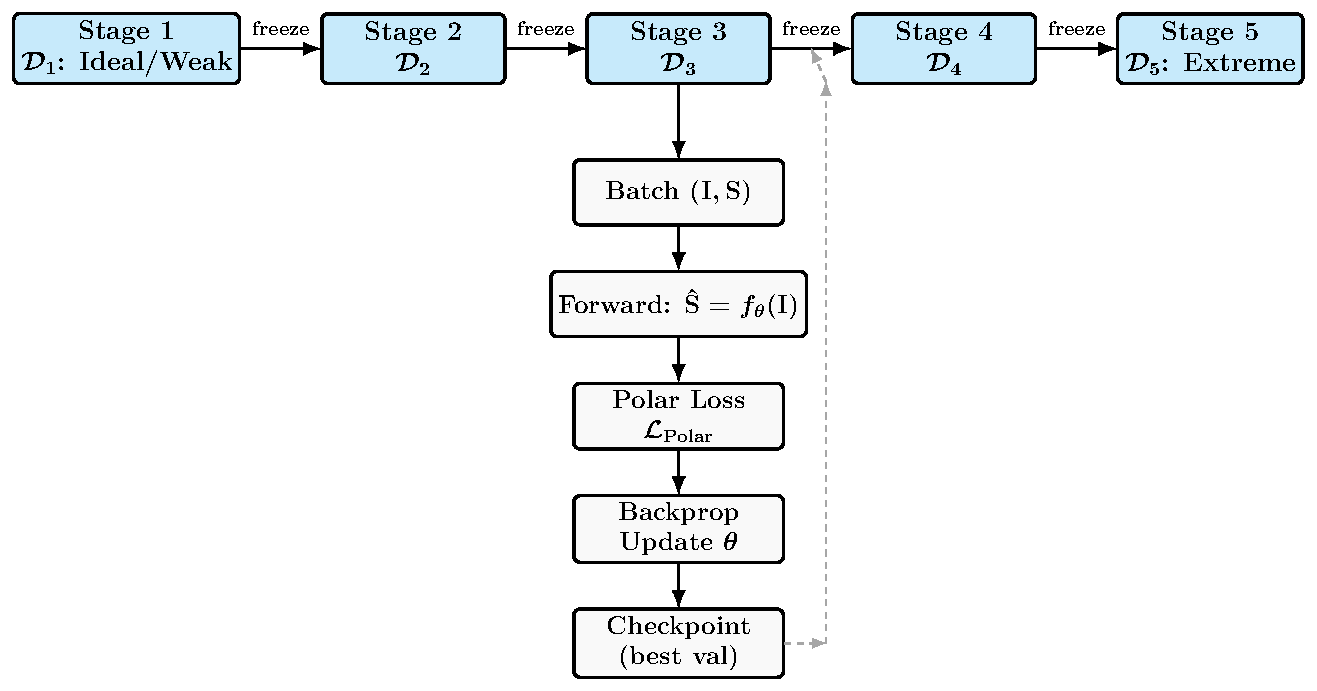
\includegraphics[width=\figdblfive]{images/neural/curriculum_training.pdf}
\caption{Curriculum learning training pipeline. Five sequential stages from ideal/very weak ($C_n^2 \approx 10^{-18}$--$10^{-17}$) to extreme ($C_n^2 = 10^{-14}$--$10^{-12}$) turbulence. Weights from each stage are frozen and transferred to the next; Polar Loss and validation-driven checkpointing are applied per stage.}
\label{fig:neural_curriculum}
\end{figure*}


% \FloatBarrier

\begin{table}[htbp]
\centering
\caption{Neural Receiver Training Configuration}
\label{tab:neural_hparams}
\small
\renewcommand{\arraystretch}{1.1}
\begin{tabularx}{\columnwidth}{l X}
\toprule
\textbf{Item} & \textbf{Configuration} \\
\midrule
Backbone used in curriculum runs & ConvNeXt-Tiny (single-channel stem adapted from ImageNet pretraining) \\
Input / output & $128 \times 128 \times 1$ intensity image $\rightarrow 8 \times 2$ I/Q outputs \\
Head & MLP: 1024 $\rightarrow$ 512 $\rightarrow$ 16; BatchNorm + LeakyReLU after first layer; Dropout (0.4) before second layer \\
Optimizer & AdamW~\cite{loshchilov2019decoupled} \\
Stage schedule & 5 curriculum stages; 100 epochs per stage \\
Batch size & 64 \\
Learning rate & $10^{-4}$ at stage 1; $5 \times 10^{-5}$ during later-stage fine-tuning \\
Weight decay / dropout & $10^{-4}$ / 0.4 \\
Scheduler & Cosine annealing at stage 1; ReduceLROnPlateau during fine-tuning stages \\
Early stopping & Patience of 20 validation checks; best-checkpoint transfer across stages \\
\bottomrule
\end{tabularx}
\end{table}

Algorithms~\ref{alg:neural_training} and~\ref{alg:neural_inference} give pseudocode for the training and inference steps.

\begin{algorithm}[!t]
\caption{Neural Receiver Training}
\label{alg:neural_training}
\KwInput{Curriculum datasets $\mathcal{D}_1, \ldots, \mathcal{D}_L$ (weak to strong turbulence), model $f_\theta$}
\KwOutput{Best checkpoint}
Initialize $f_\theta$ (ConvNeXt/EfficientNet backbone, single-channel input, symbol head)\;
\For{each stage $\ell = 1,\dots,L$}{
\If{$\ell > 1$}{
Load weights from the best checkpoint of stage $\ell-1$\;
}
\For{each epoch}{
Sample batch $(\mathbf{I}, \mathbf{S})$ and predict $\hat{\mathbf{S}} = f_\theta(\mathbf{I})$\;
Compute Polar Loss, backpropagate, and update $\theta$\;
Validate, save the best checkpoint, and early stop if validation stalls\;
}
}
\Return{Best checkpoint}
\end{algorithm}

Training thus proceeds in curriculum order: for each stage the optimizer minimizes the polar loss on batches drawn from that stage's turbulence range, validation tracks generalization, the best weights initialize the next stage, and early stopping prevents overfitting when the validation plateau persists.

\begin{algorithm}[!t]
\caption{Neural Receiver Inference}
\label{alg:neural_inference}
\KwInput{Trained model $f_\theta$, test set $\mathcal{D}^{test}$ (intensity images + labels)}
\KwOutput{BER, SER}
Load the best checkpoint and set $f_\theta$ to evaluation mode\;
\For{each batch $(\mathbf{I}, \mathbf{S})$ in $\mathcal{D}^{test}$}{
$\hat{\mathbf{S}} \leftarrow f_\theta(\mathbf{I})$ (no gradient)\;
}
Demodulate predicted and target symbols to bits and compute BER and SER\;
\Return{BER, SER}
\end{algorithm}

At inference time the model is frozen; batches of intensity maps are mapped to symbol estimates without any pilot or matrix inversion, hard/soft demapping yields bits, and BER/SER summarize end-to-end accuracy on the held-out test split.

% \FloatBarrier
%==============================================================================
% IV. RESULTS
%==============================================================================
\section{Results}
\label{sec:results}

The classical baseline is validated first. Table~\ref{tab:link_params} gives the full simulation setup: eight-mode OAM-multiplexed QPSK at 1550~nm over 1~km, turbulence modeled via split-step Fourier propagation with Kolmogorov phase screens~\cite{schmidt2010numerical, andrews2005laser}. At each $C_n^2$ operating point, results are averaged over 2 independent channel realizations of 3332 bits each.

Fig.~\ref{fig:mode_overlap} quantifies how overlap between each propagated mode and its undisturbed reference falls as $C_n^2$ increases. The decline is fairly steep across modes and sets in somewhat sooner for higher-order modes, foreshadowing the BER transition observed below.

\begin{figure}[htbp]
\centering
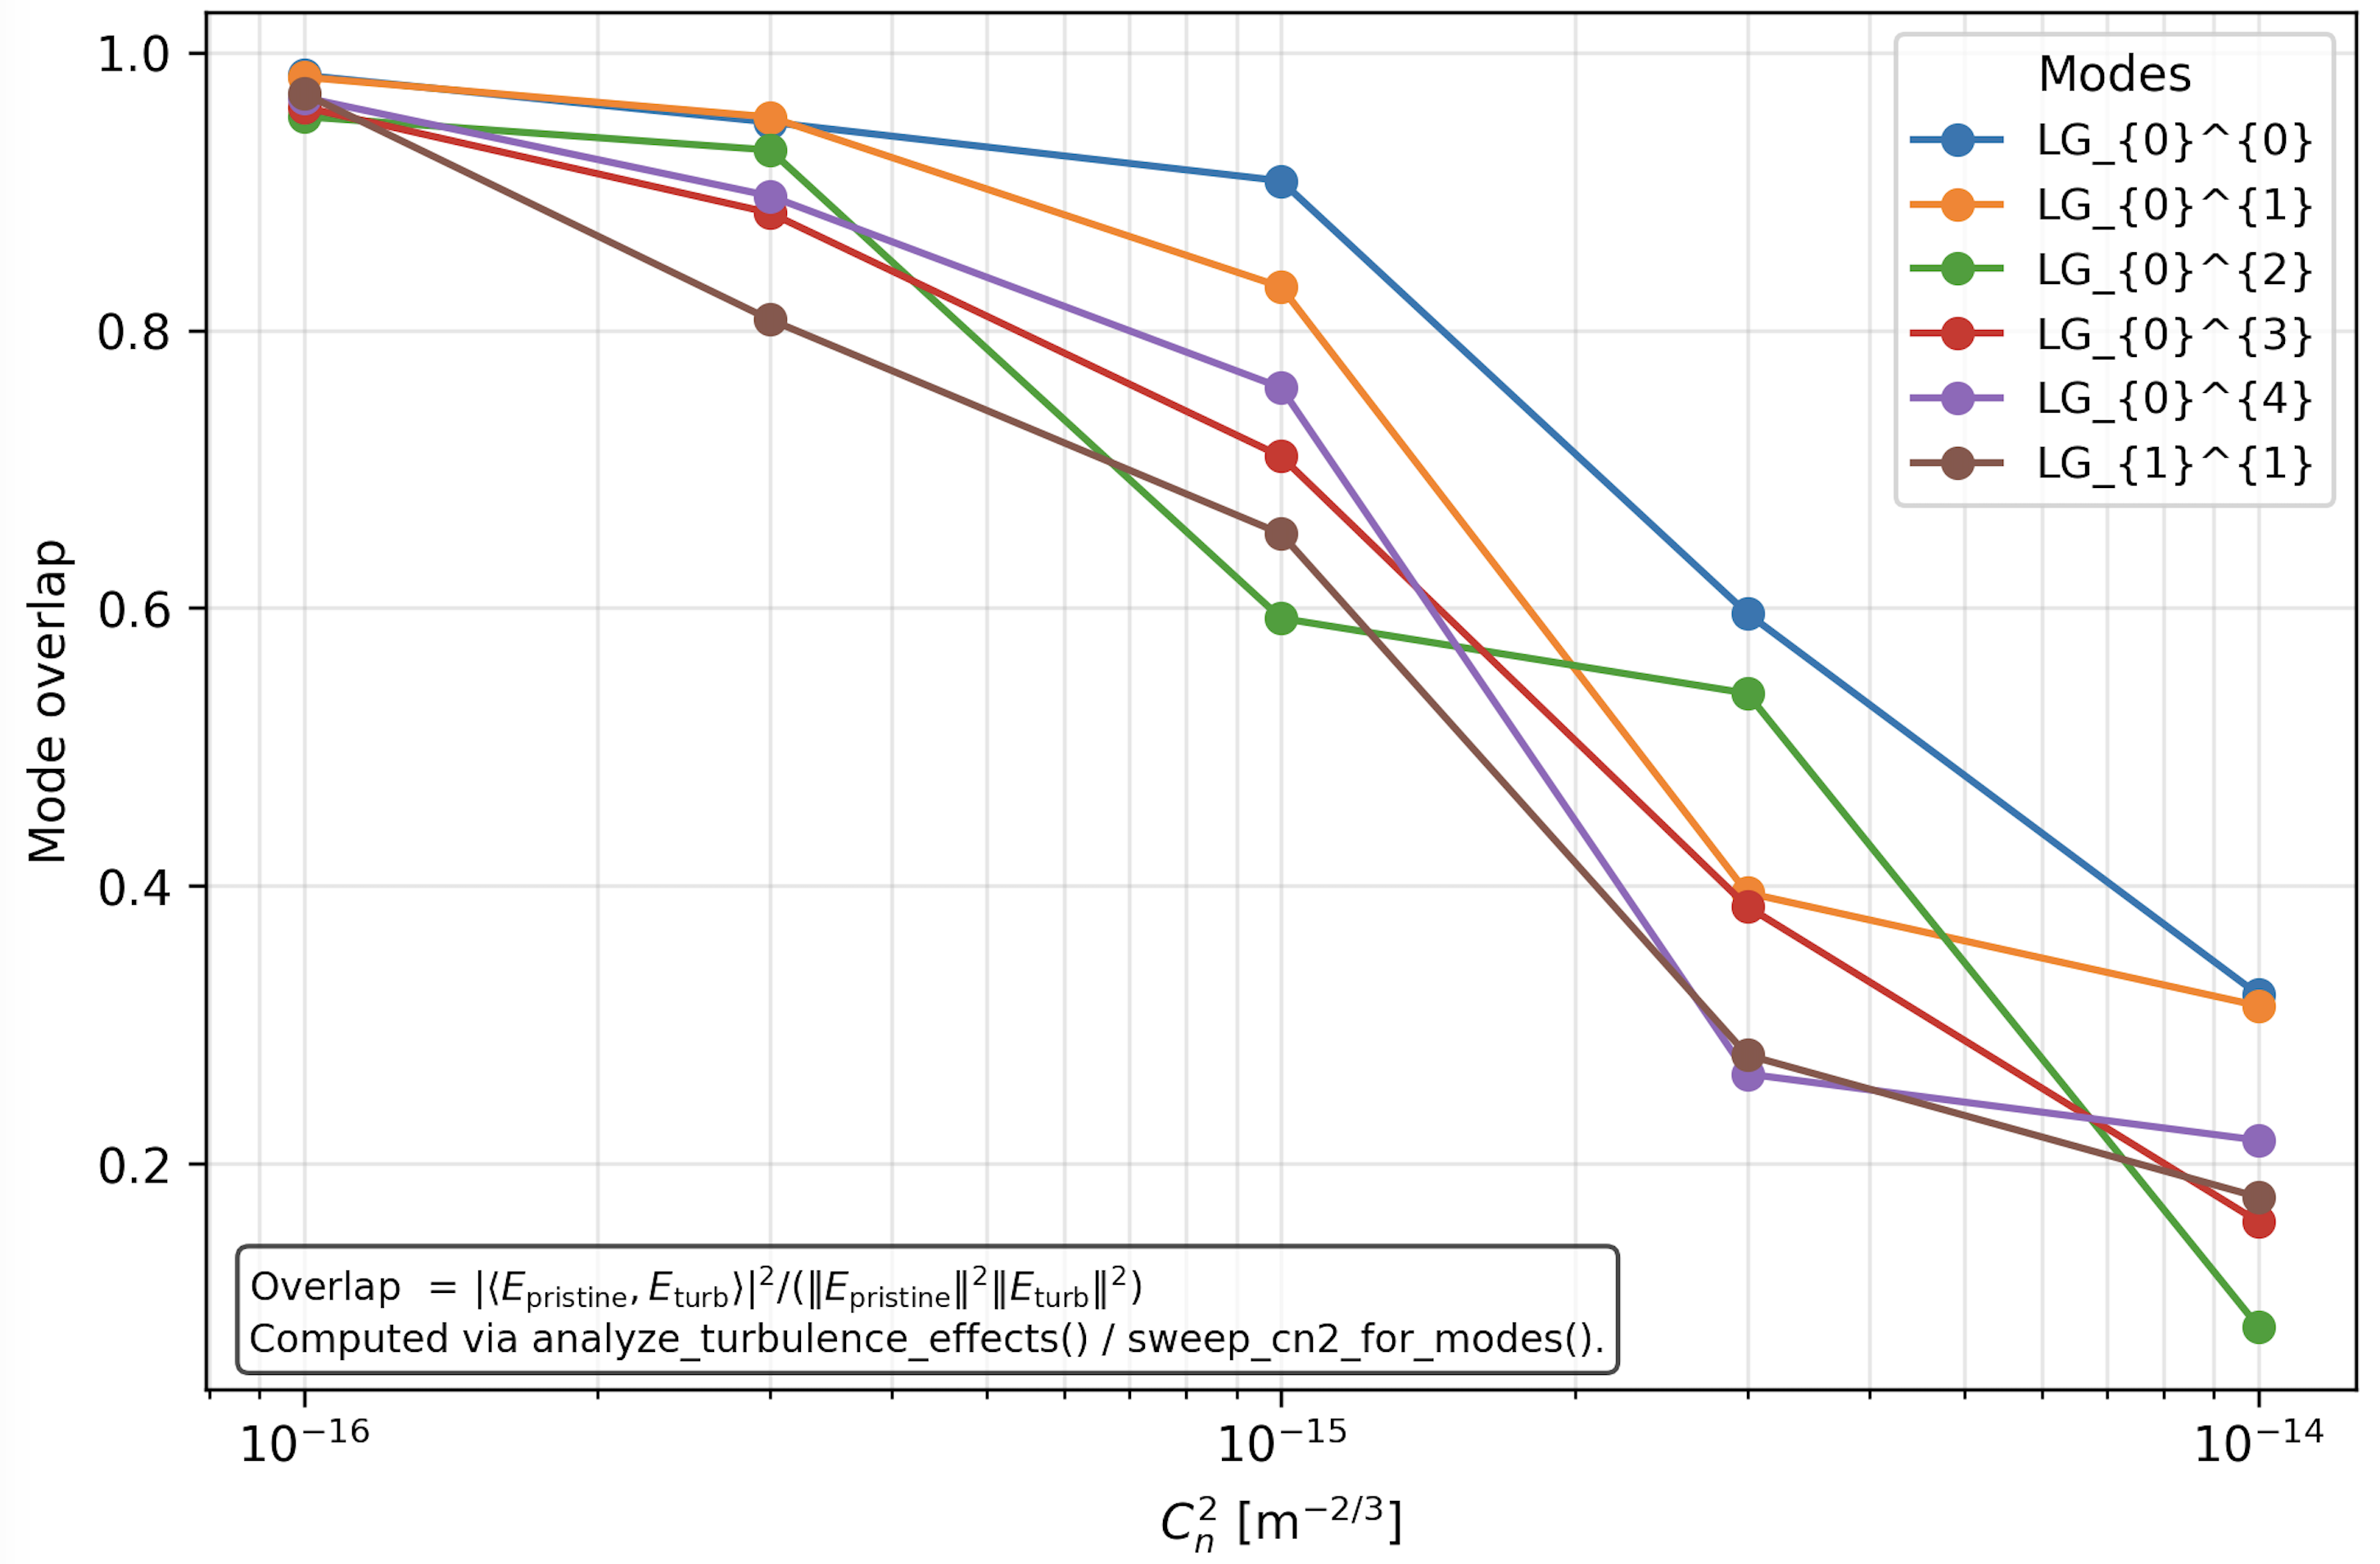
\includegraphics[width=\figcol]{images/classical/modal_overlap_vs_cn2.png}
\caption{Mode overlap versus turbulence strength $C_n^2$. Each curve shows the overlap of a propagated LG mode with its pristine counterpart. The decline quantifies the loss of modal fidelity that drives inter-modal crosstalk and BER degradation.}
\label{fig:mode_overlap}
\end{figure}


The BER-versus-$C_n^2$ curve in Fig.~\ref{fig:ber_main} shows a consistent pattern. In weak turbulence ($C_n^2 \lesssim 10^{-16}$), BER remains near zero and LDPC gain is clear. In the transition region ($C_n^2 \approx 10^{-15}$--$10^{-14}$), modal coupling rises quickly, pre- and post-LDPC BER both increase, and the gap between them narrows as $\kappa(\hat{\mathbf{H}})$ grows from about 2 to about 17. Beyond $10^{-14}$, the curves merge near 0.5, which is close to random guessing. Table~\ref{tab:ber_key} gives BER and $\kappa(\hat{\mathbf{H}})$ at representative operating points, and Fig.~\ref{fig:channel_matrices} shows the evolution of $|\hat{\mathbf{H}}|$ from ideal to extreme turbulence.

\begin{figure}[htbp]
\centering
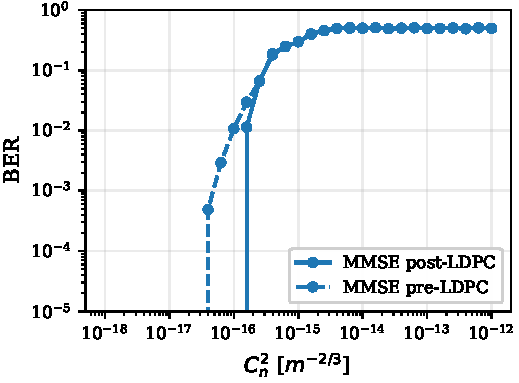
\includegraphics[width=\figcol]{images/classical/pre_post_ldpc_ber.pdf}
\caption{Classical baseline BER versus turbulence strength $C_n^2$. Pre-LDPC (dashed) and post-LDPC (solid) curves show coding gain in weak turbulence and its collapse in the transition regime.}
\label{fig:ber_main}
\end{figure}

\begin{table}[htbp]
\centering
\caption{Classical Baseline BER at Representative $C_n^2$ (SNR = 35~dB)}
\label{tab:ber_key}
\small
\renewcommand{\arraystretch}{1.1}
\begin{tabular}{c c c c}
\toprule
$C_n^2$ (m$^{-2/3}$) & Pre-LDPC BER & Post-LDPC BER & $\kappa(\hat{\mathbf{H}})$ \\
\midrule
$10^{-18}$ & $<10^{-4}$ & $<10^{-4}$ & 1.01 \\
$10^{-17}$ & $<10^{-4}$ & $<10^{-4}$ & 1.02 \\
$10^{-16}$ & $<10^{-4}$ & 0.011$^\dagger$ & 1.11 \\
$10^{-15}$ & 0.30 & 0.30 & 2.95 \\
$10^{-14}$ & 0.50 & 0.50 & 17.4 \\
$10^{-13}$ & 0.49 & 0.49 & 17.0 \\
$10^{-12}$ & 0.50 & 0.50 & 22.8 \\
\bottomrule
\end{tabular}
\vspace{1mm}
{\footnotesize $^\dagger$At $C_n^2=10^{-16}$, zero hard-decision pre-LDPC errors were observed across 2 channel realizations (6{,}664 coded bits). The nonzero post-LDPC figure reflects marginal soft LLR quality at this operating point and is statistically unreliable at this sample size; additional realizations are needed for a reliable post-LDPC estimate in this regime.}
\end{table}

\begin{figure*}[!t]
\centering
\setlength{\tabcolsep}{\subfiggap}
\begin{tabular}{@{}c@{\hspace{\subfiggap}}c@{\hspace{\subfiggap}}c@{}}
\subfloat[Ideal.\label{fig:ch_ideal}]{%
  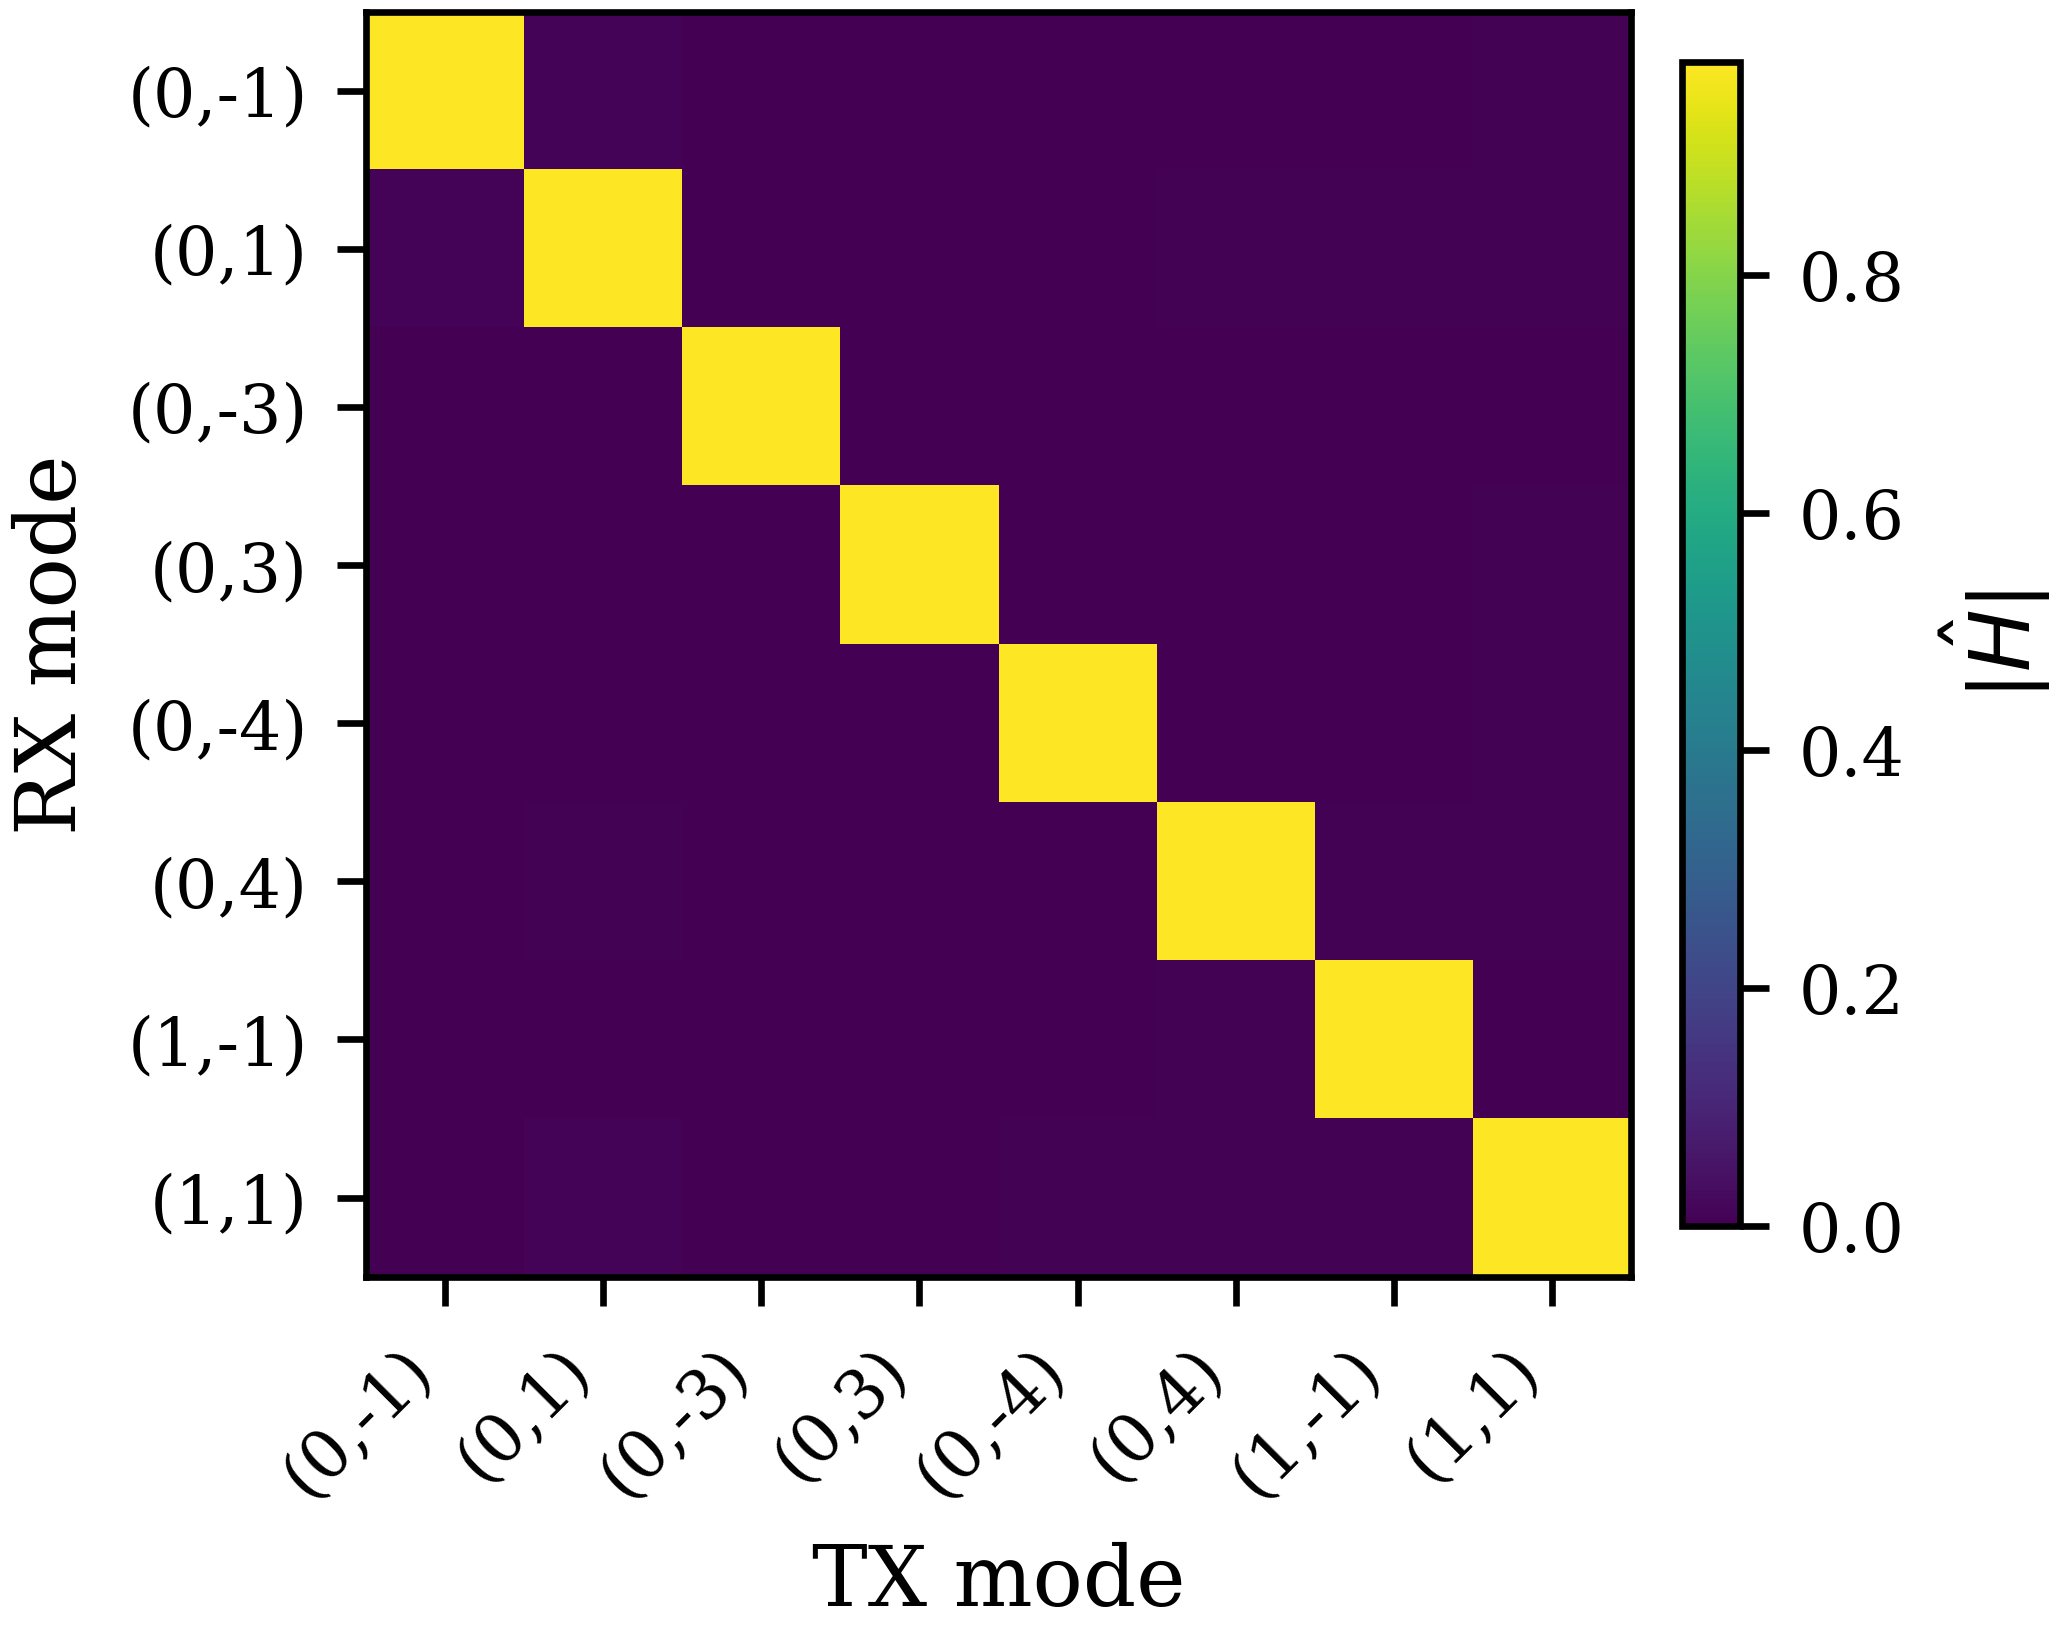
\includegraphics[width=\subfigw]{images/classical/ideal_channel_matrix.png}%
} &
\subfloat[Weak.\label{fig:ch_weak}]{%
  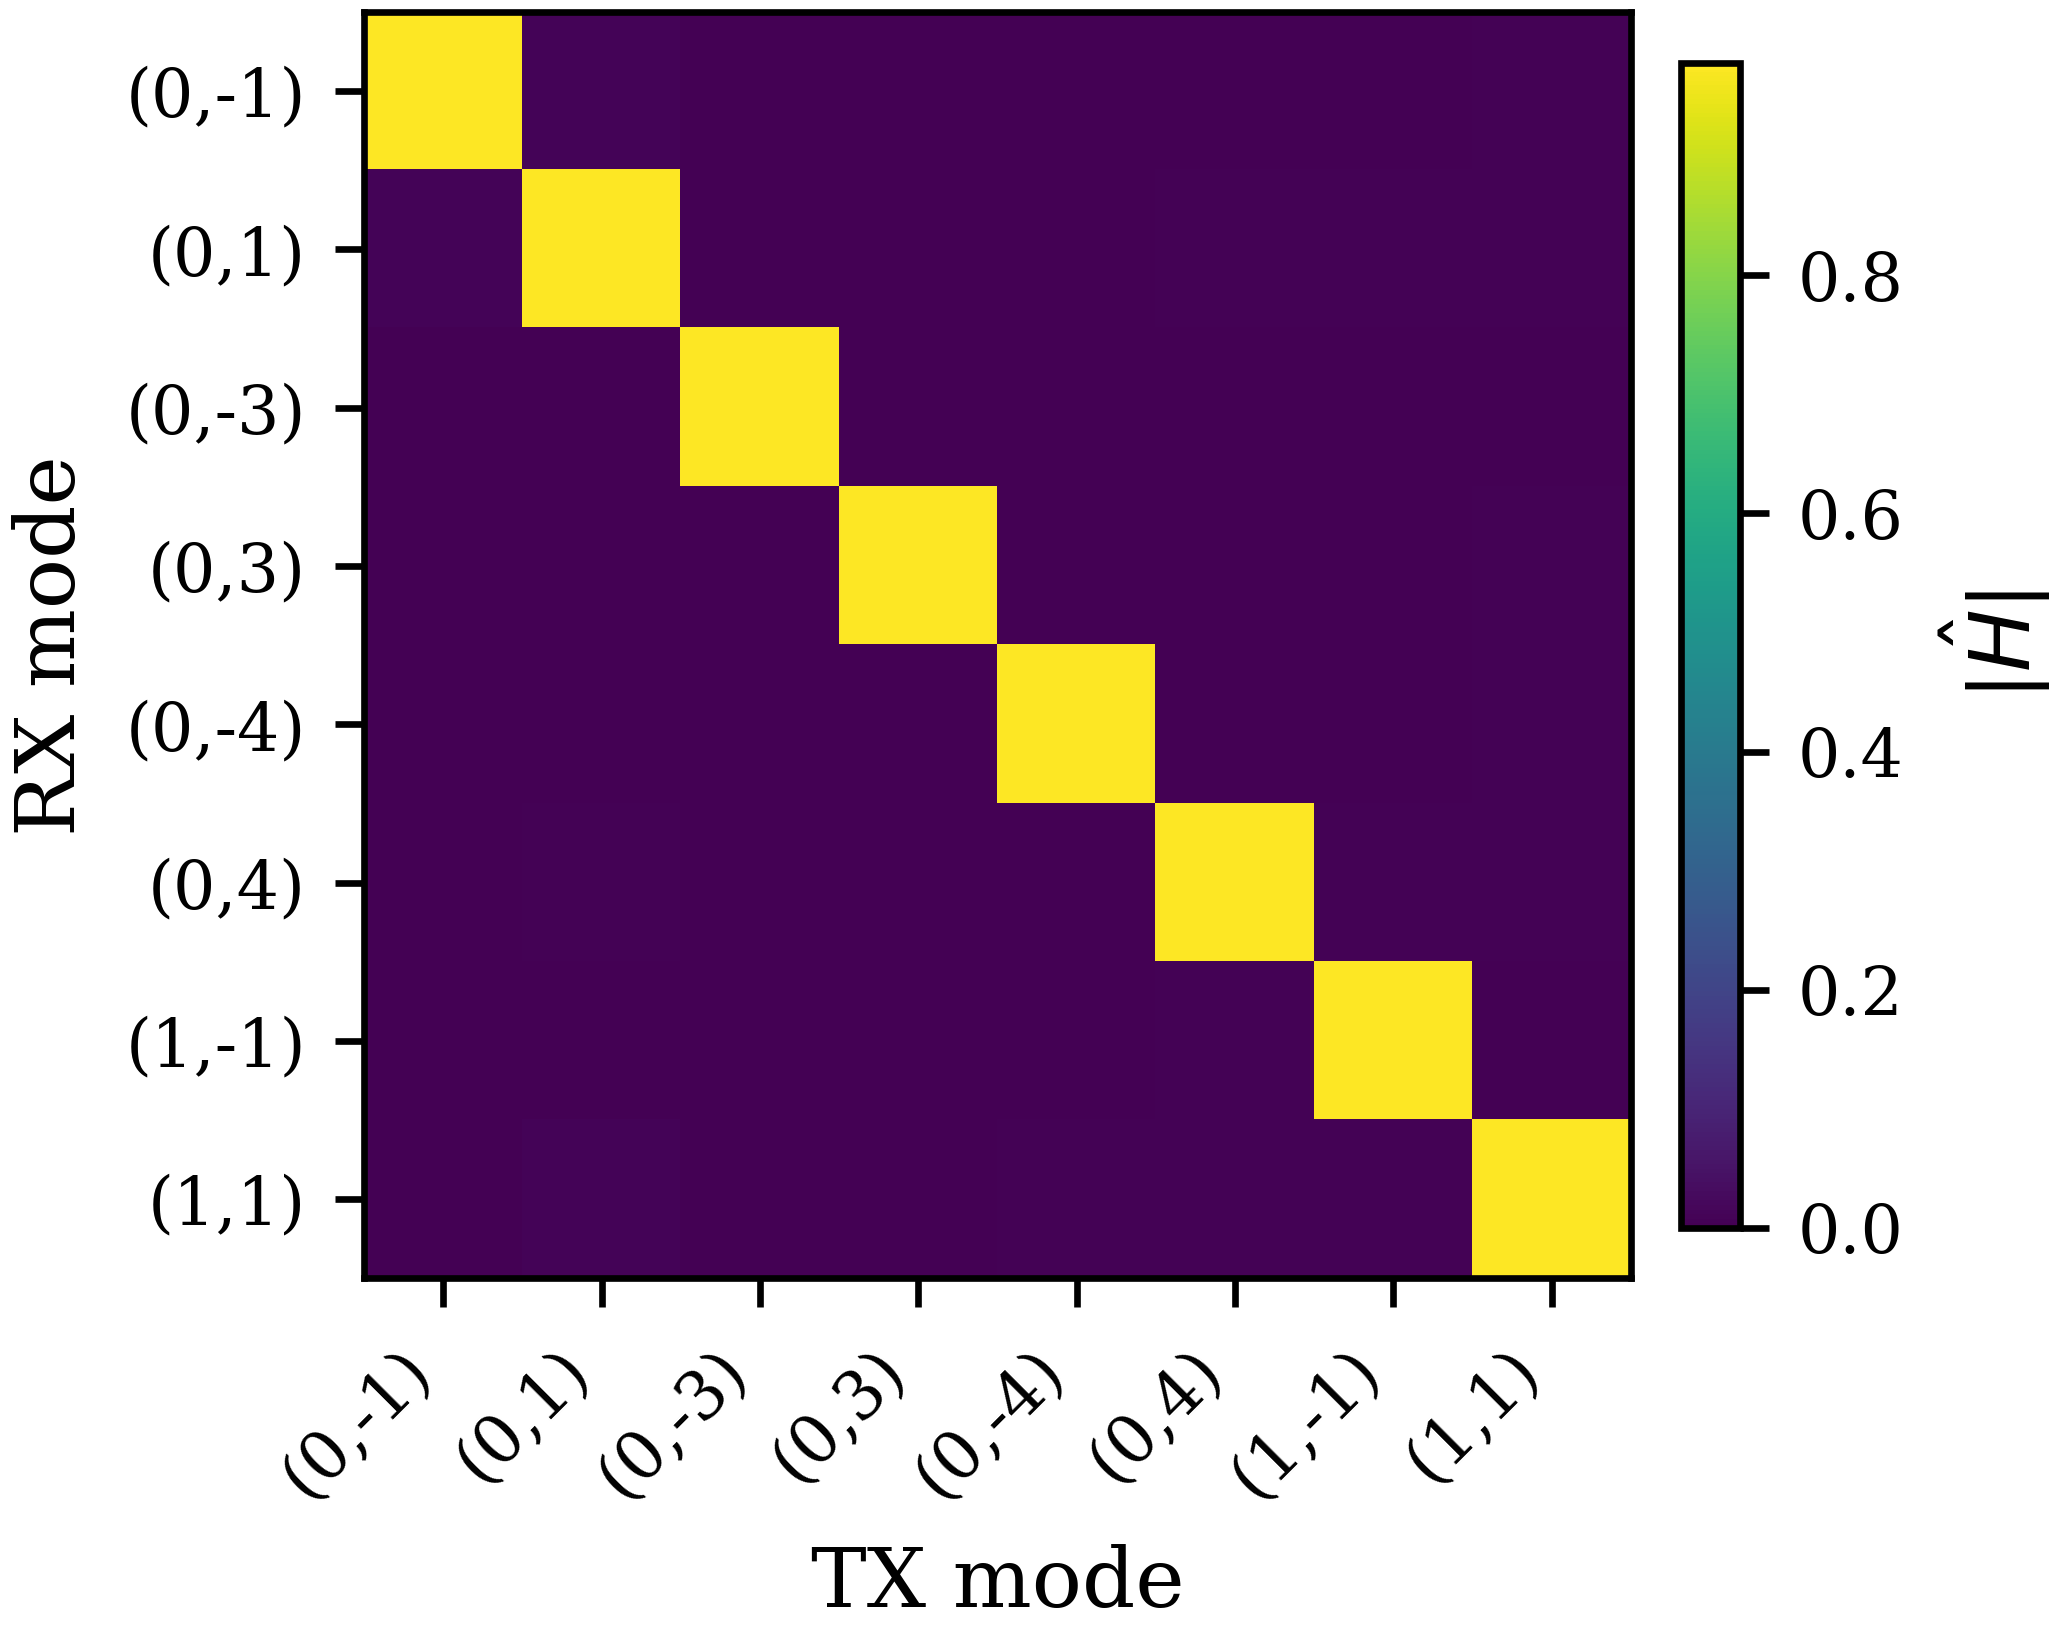
\includegraphics[width=\subfigw]{images/classical/weak_channel_matrix.png}%
} &
\subfloat[Moderate.\label{fig:ch_moderate}]{%
  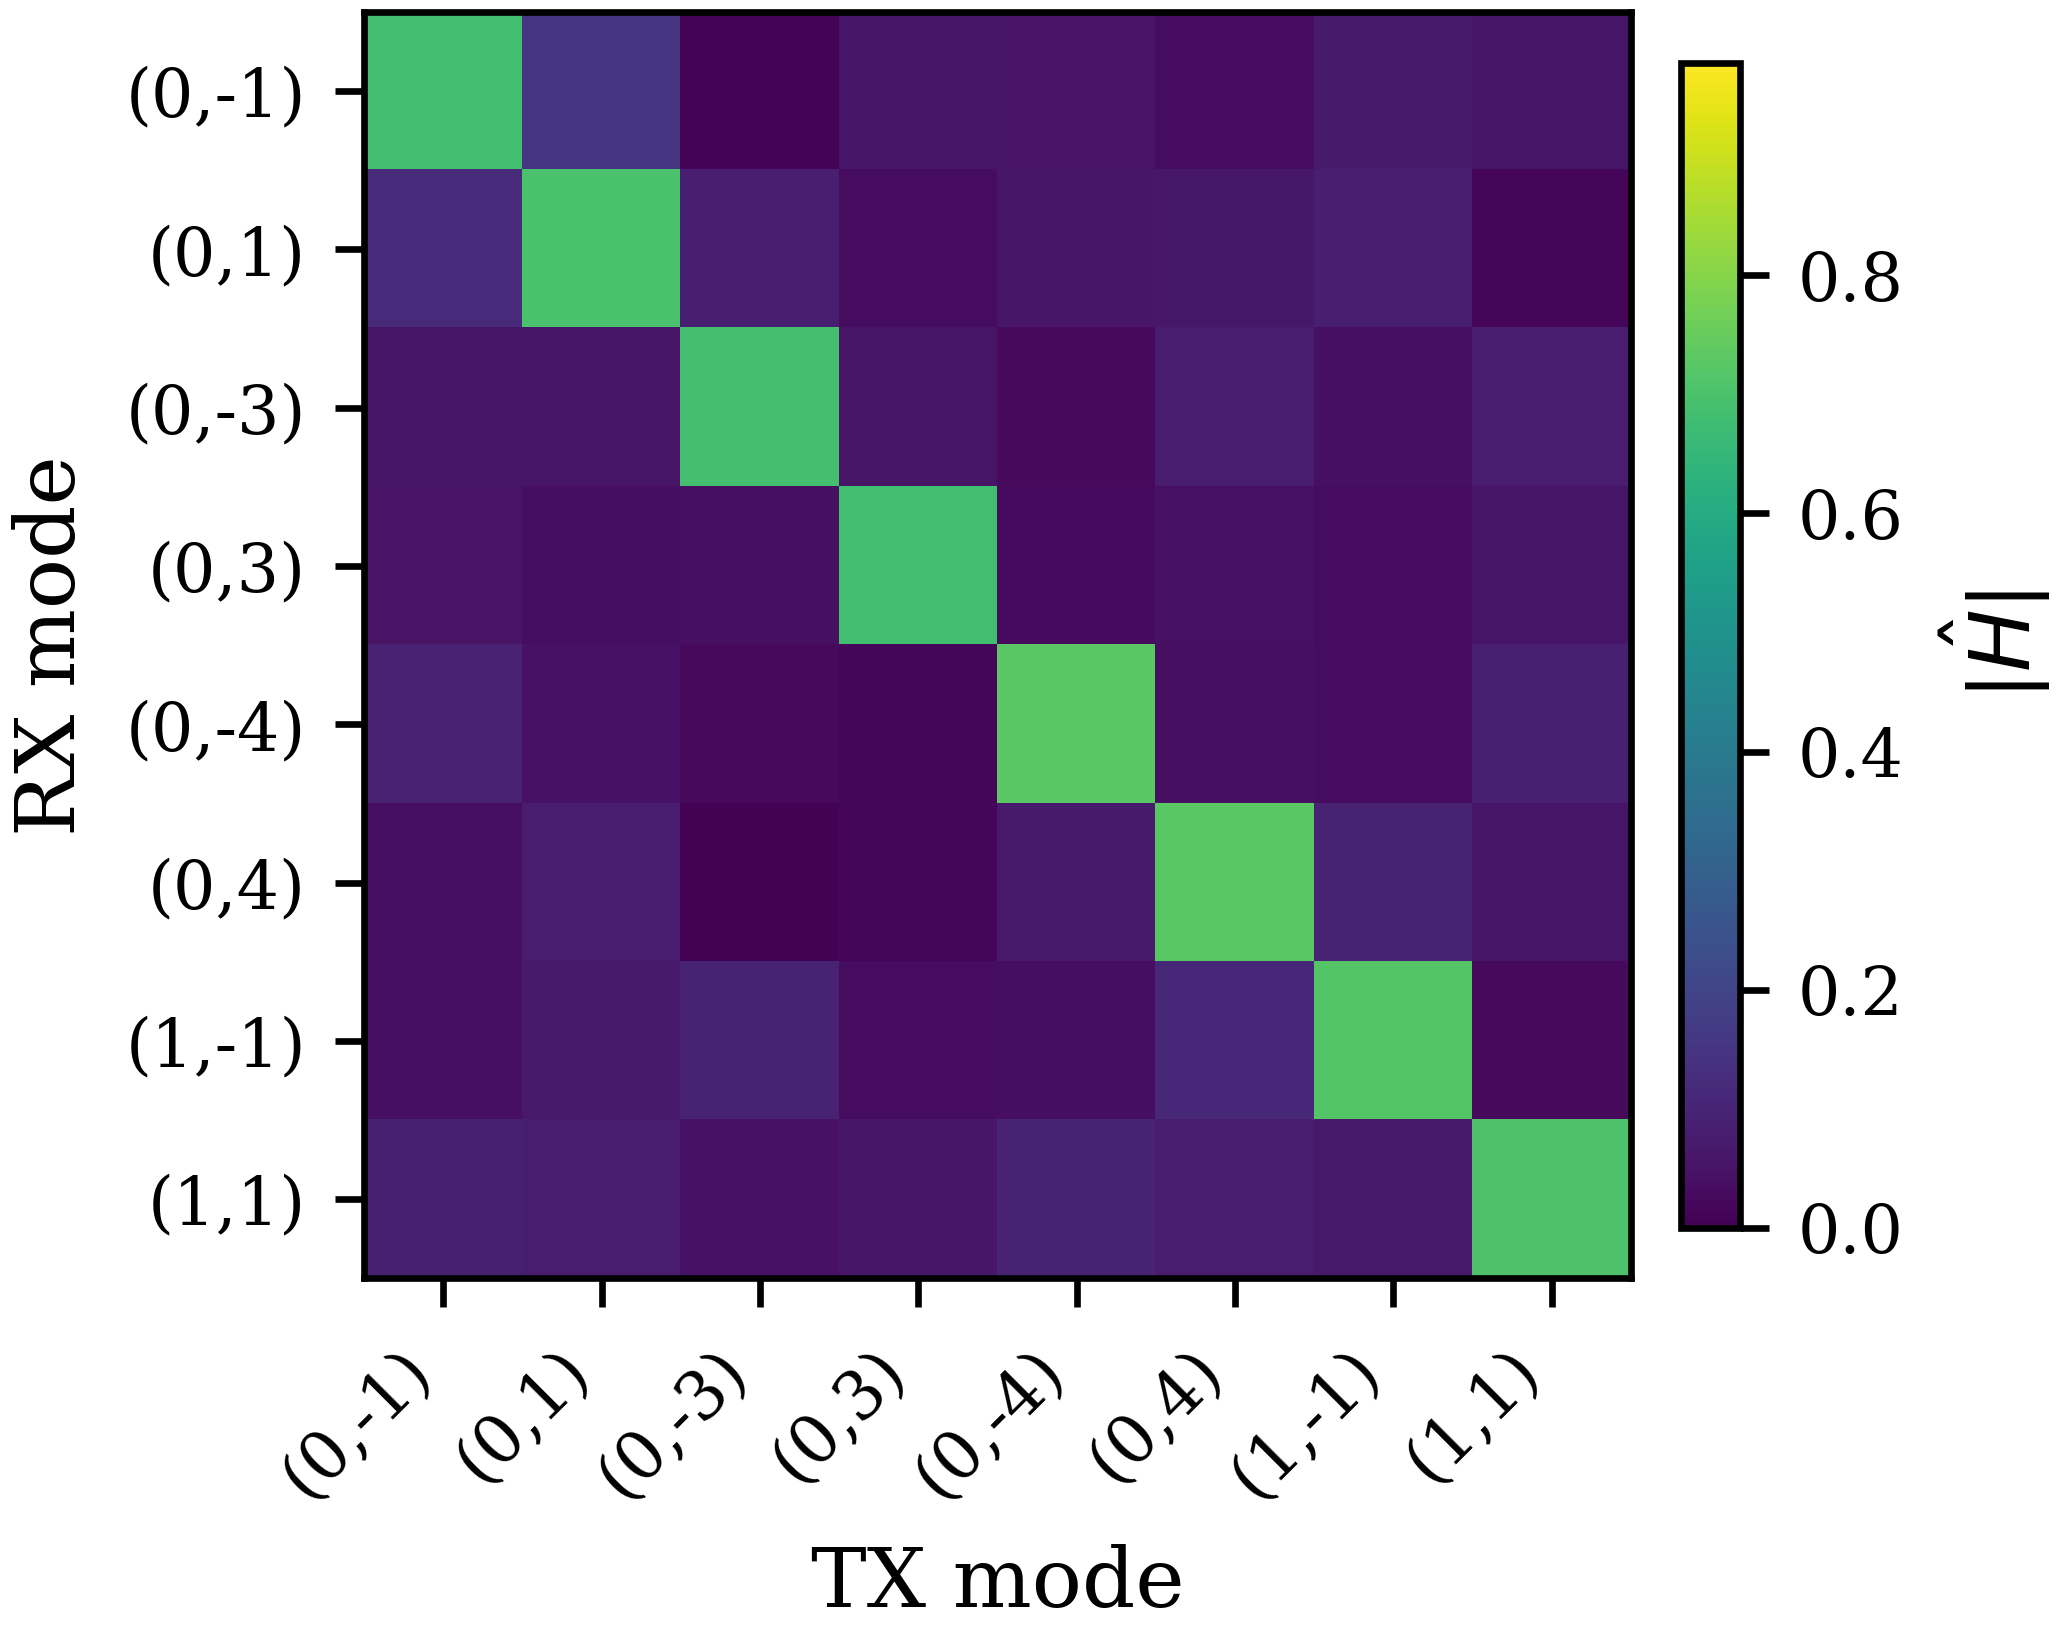
\includegraphics[width=\subfigw]{images/classical/moderate_channel_matrix.png}%
}
\end{tabular}\\[0.8ex]
\makebox[\textwidth][c]{%
\begin{tabular}{@{}c@{\hspace{\subfiggap}}c@{}}
\subfloat[Transition/strong.\label{fig:ch_transition}]{%
  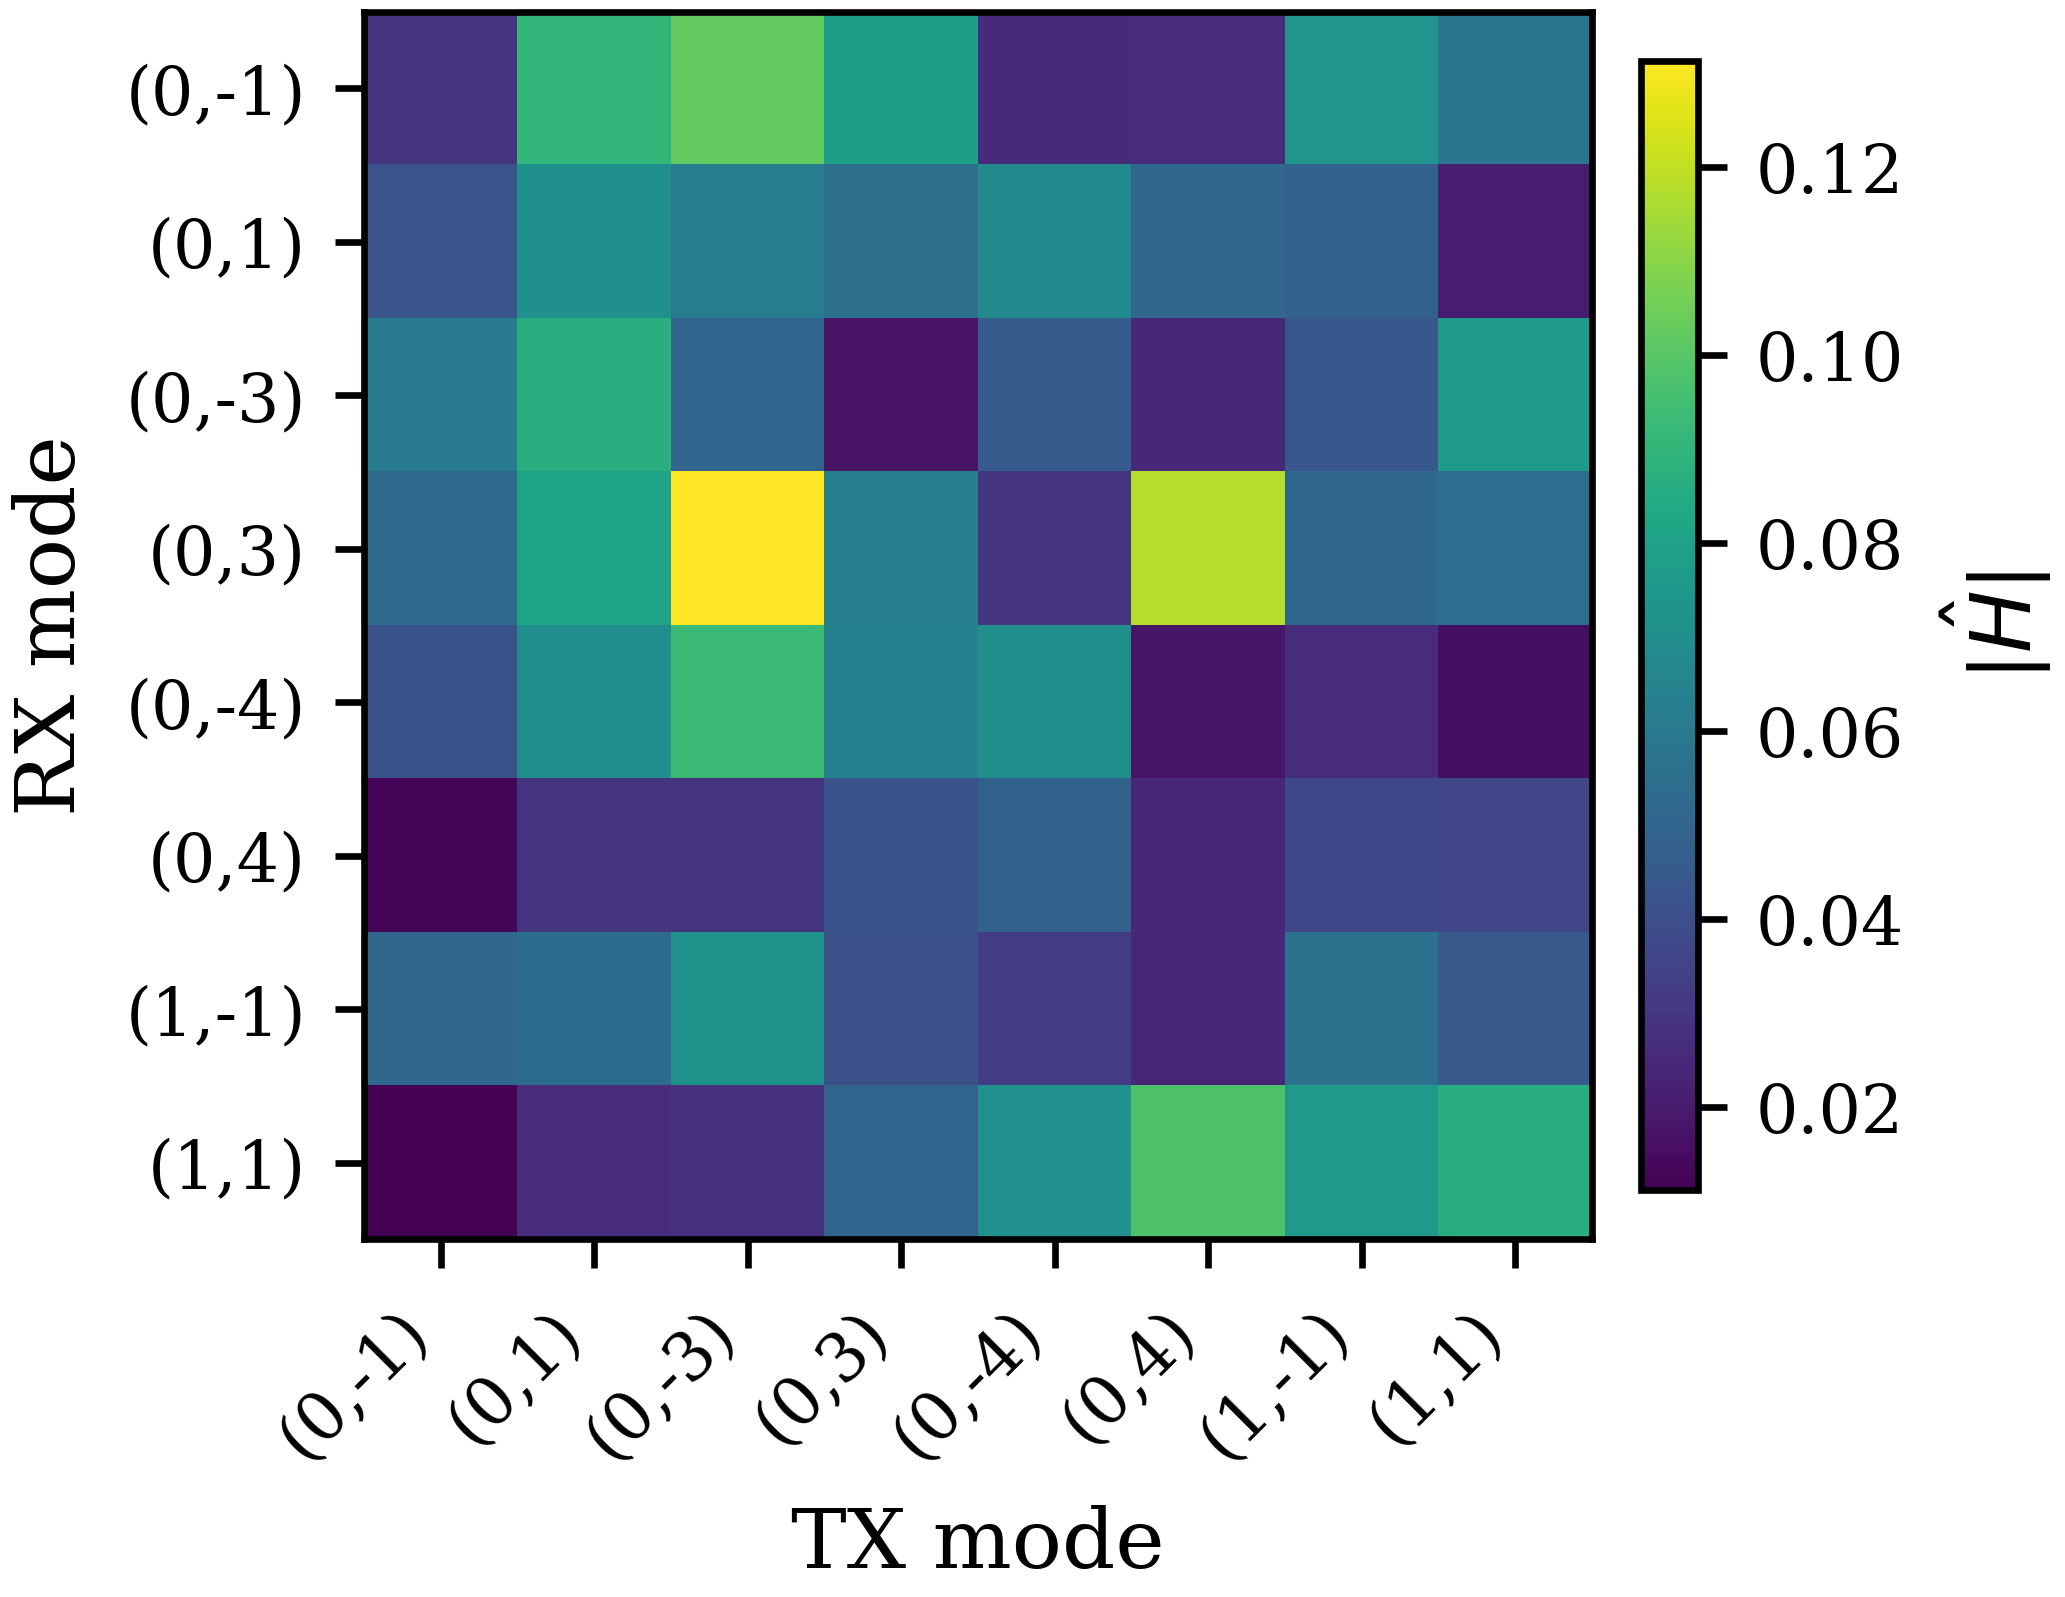
\includegraphics[width=0.317\textwidth]{images/classical/transition_channel_matrix.png}%
} &
\subfloat[Extreme.\label{fig:ch_extreme}]{%
  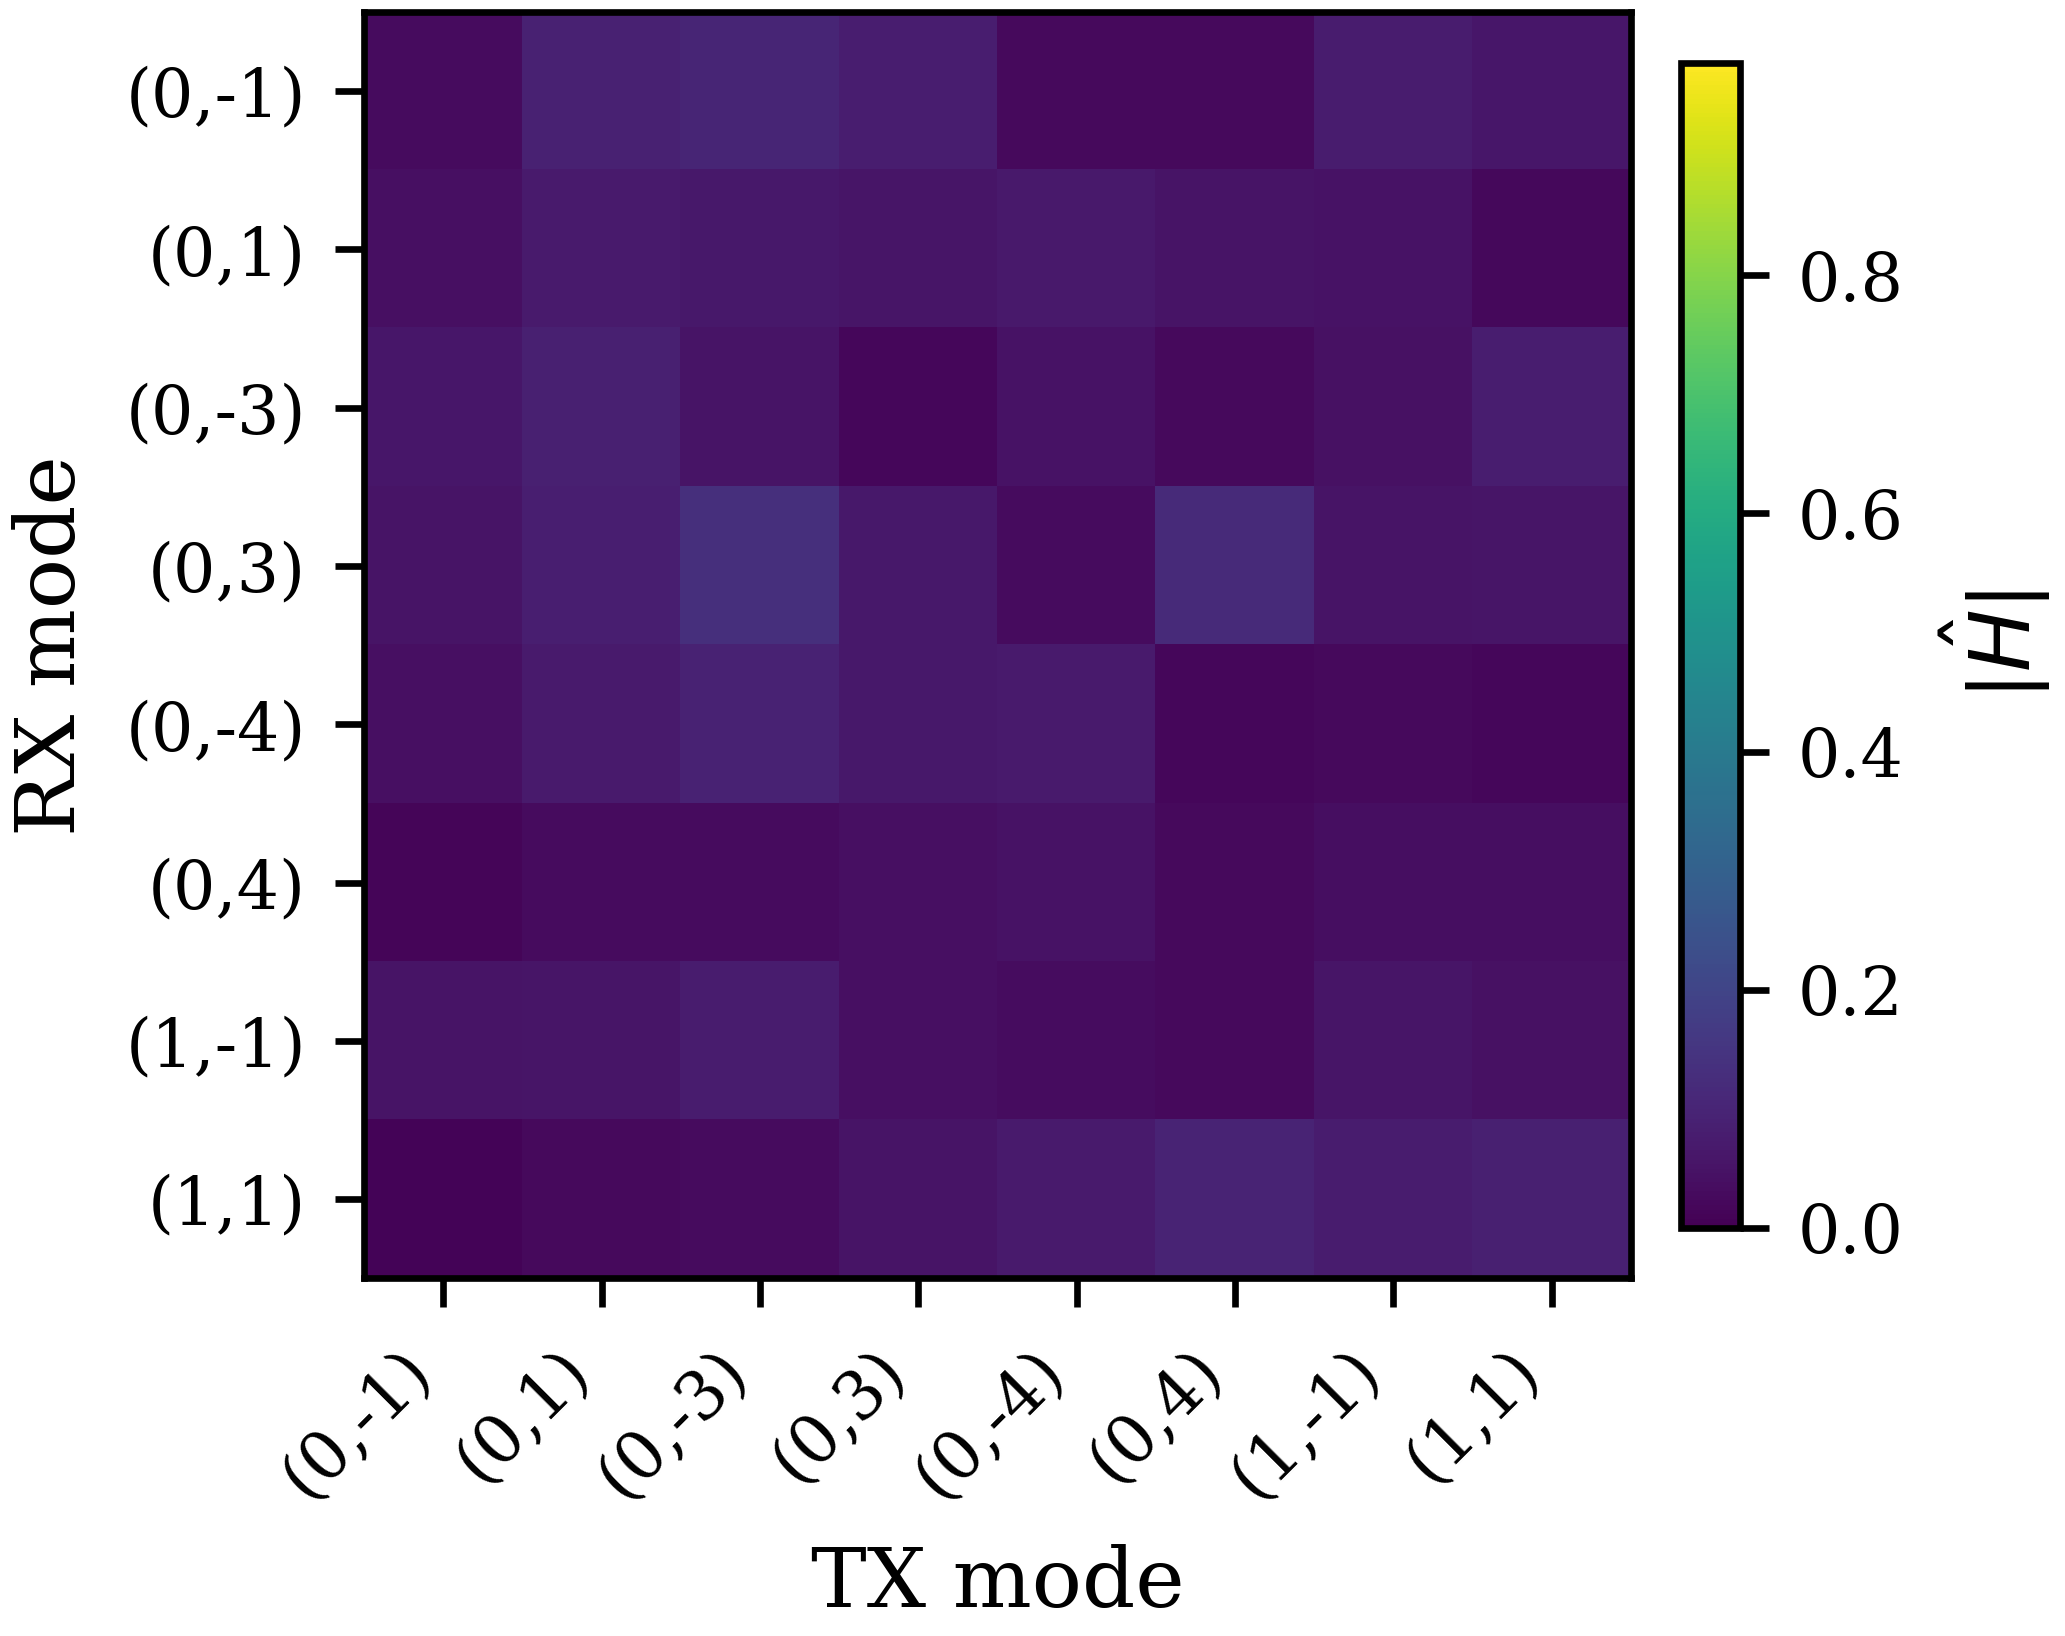
\includegraphics[width=\subfigw]{images/classical/extreme_channel_matrix.png}%
}
\end{tabular}
}
\caption{Estimated channel matrix magnitude $|\hat{\mathbf{H}}|$ across representative classical operating regimes. (a) Ideal ($C_n^2 = 10^{-18}$): near-perfect diagonal structure; (b) weak: strong diagonal dominance with limited coupling; (c) moderate: off-diagonal mixing begins to emerge; (d) transition/strong: modal structure degrades rapidly; (e) extreme: the matrix loses clear diagonal dominance and approaches diffuse coupling.}
\label{fig:channel_matrices}
\end{figure*}


Three points are worth emphasizing. LDPC gain is substantial only in weak turbulence; once $C_n^2$ passes roughly $10^{-15}$, the pre- and post-decoding curves merge, which suggests the soft information is too corrupted to recover. The rise in ill-conditioning, with $\kappa(\hat{\mathbf{H}})$ moving from near unity to beyond 17, tracks the BER increase closely and is consistent with MMSE noise amplification as the channel matrix degrades~\cite{kay1993fundamentals, ren2014mimo_oam}. Beyond $10^{-14}$, the matrices lose clear diagonal structure and BER settles near 0.5, making recovery effectively infeasible for this receiver design. Table~\ref{tab:performance_summary} summarizes this regime behavior.

With the classical failure pattern established, the question becomes how the curriculum-trained neural receiver fares under the same conditions.

The neural receiver was then run across the same five regimes. Fig.~\ref{fig:neural_stage_ber_all} plots BER across all five stages, and Fig.~\ref{fig:neural_stage_constellation_progression} shows how the received constellation changes from ideal to extreme conditions.

\begin{figure*}[!t]
\centering
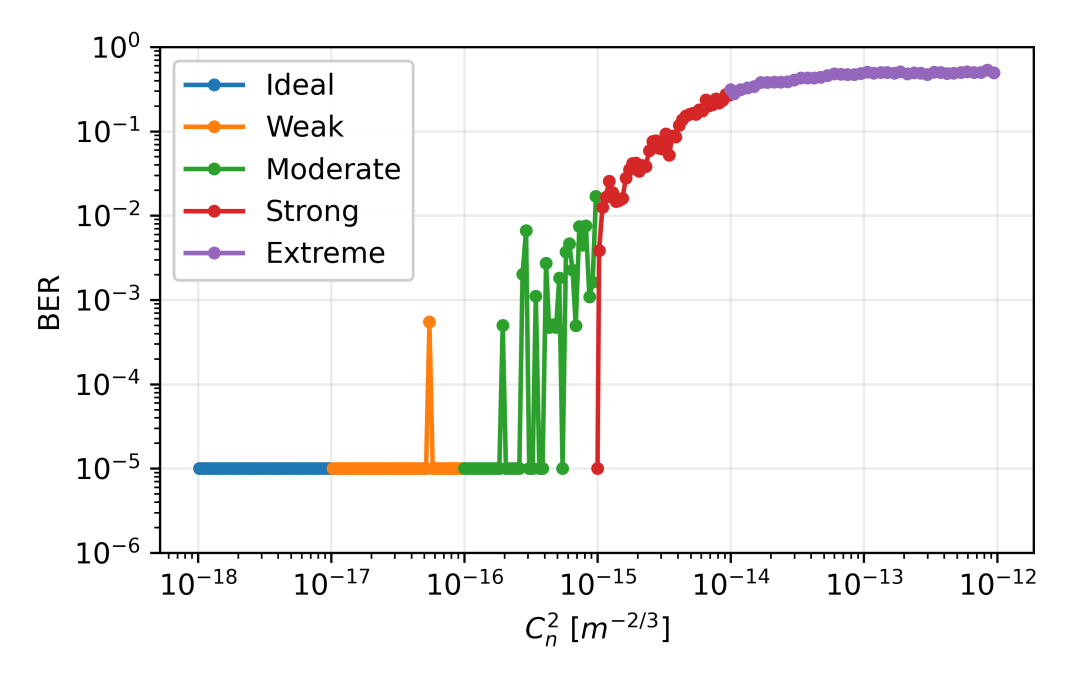
\includegraphics[width=\figdblnine]{images/neural/results/merged_ber_lvl1_to_lvl5_same_mixed_model.png}
\caption{Neural receiver BER across all five curriculum stages, same mixed model. Floor-level performance holds through the ideal and weak regimes; moderate conditions start to introduce occasional excursions; the strong interval pushes BER into $10^{-2}$--$10^{-1}$; and by the extreme regime the model is largely guessing.}
\label{fig:neural_stage_ber_all}
\end{figure*}

\begin{figure*}[!t]
\centering
\setlength{\tabcolsep}{\subfiggap}
\begin{tabular}{@{}c@{\hspace{\subfiggap}}c@{\hspace{\subfiggap}}c@{}}
\subfloat[Ideal.\label{fig:neural_const_ideal}]{%
  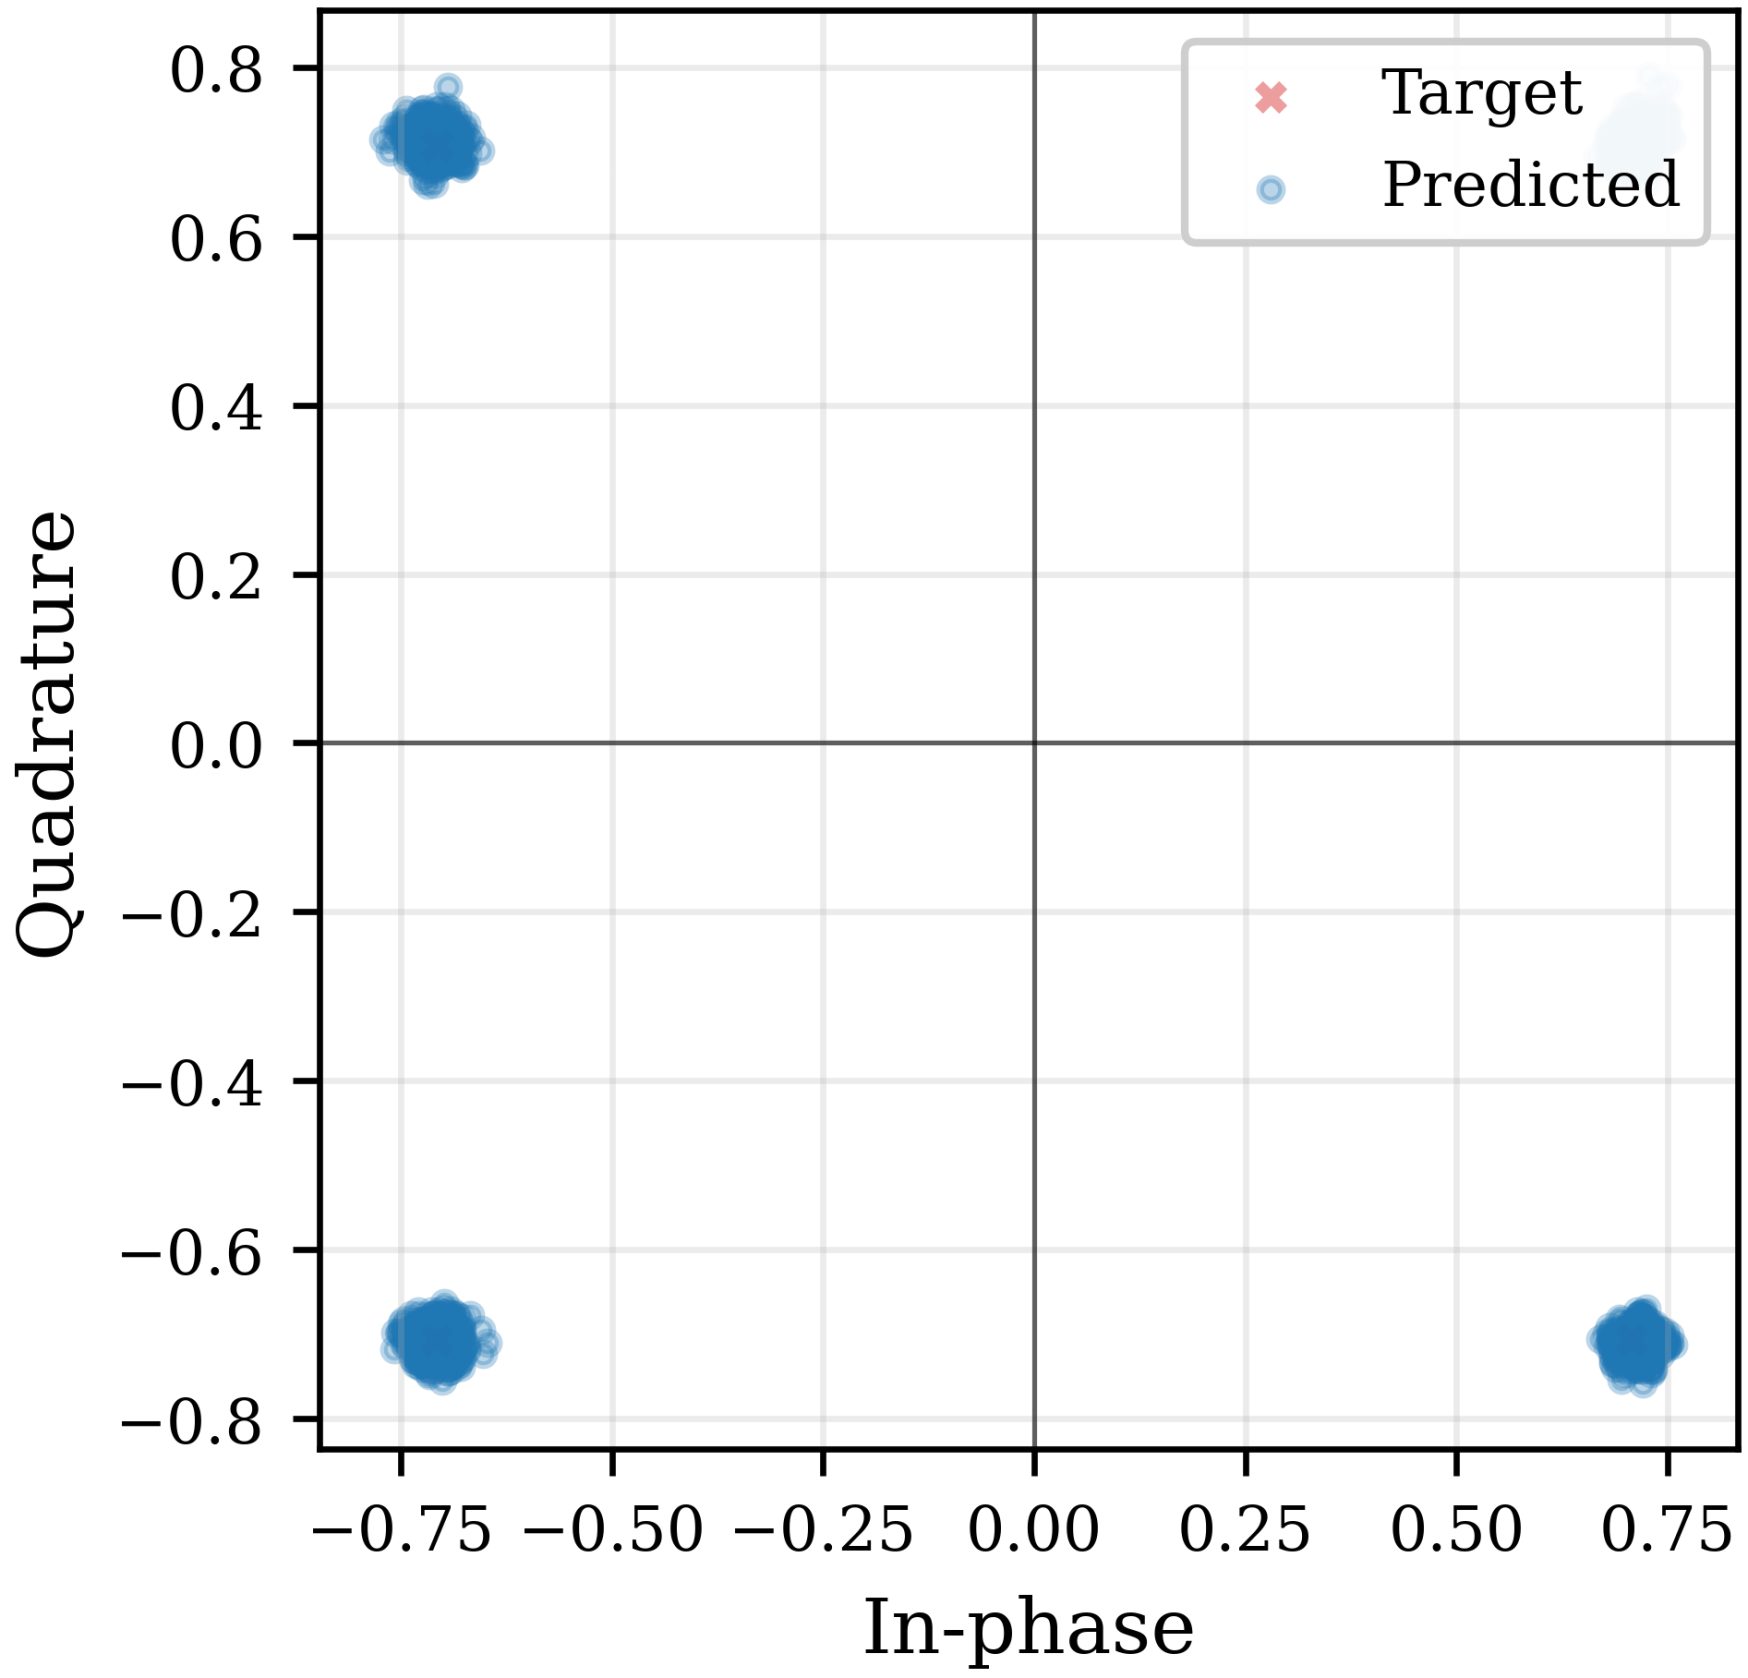
\includegraphics[width=\subfigw]{images/neural/results/cnn_constellation_convnext_tiny_curriculum_lvl1_ideal.png}%
} &
\subfloat[Weak.\label{fig:neural_const_weak}]{%
  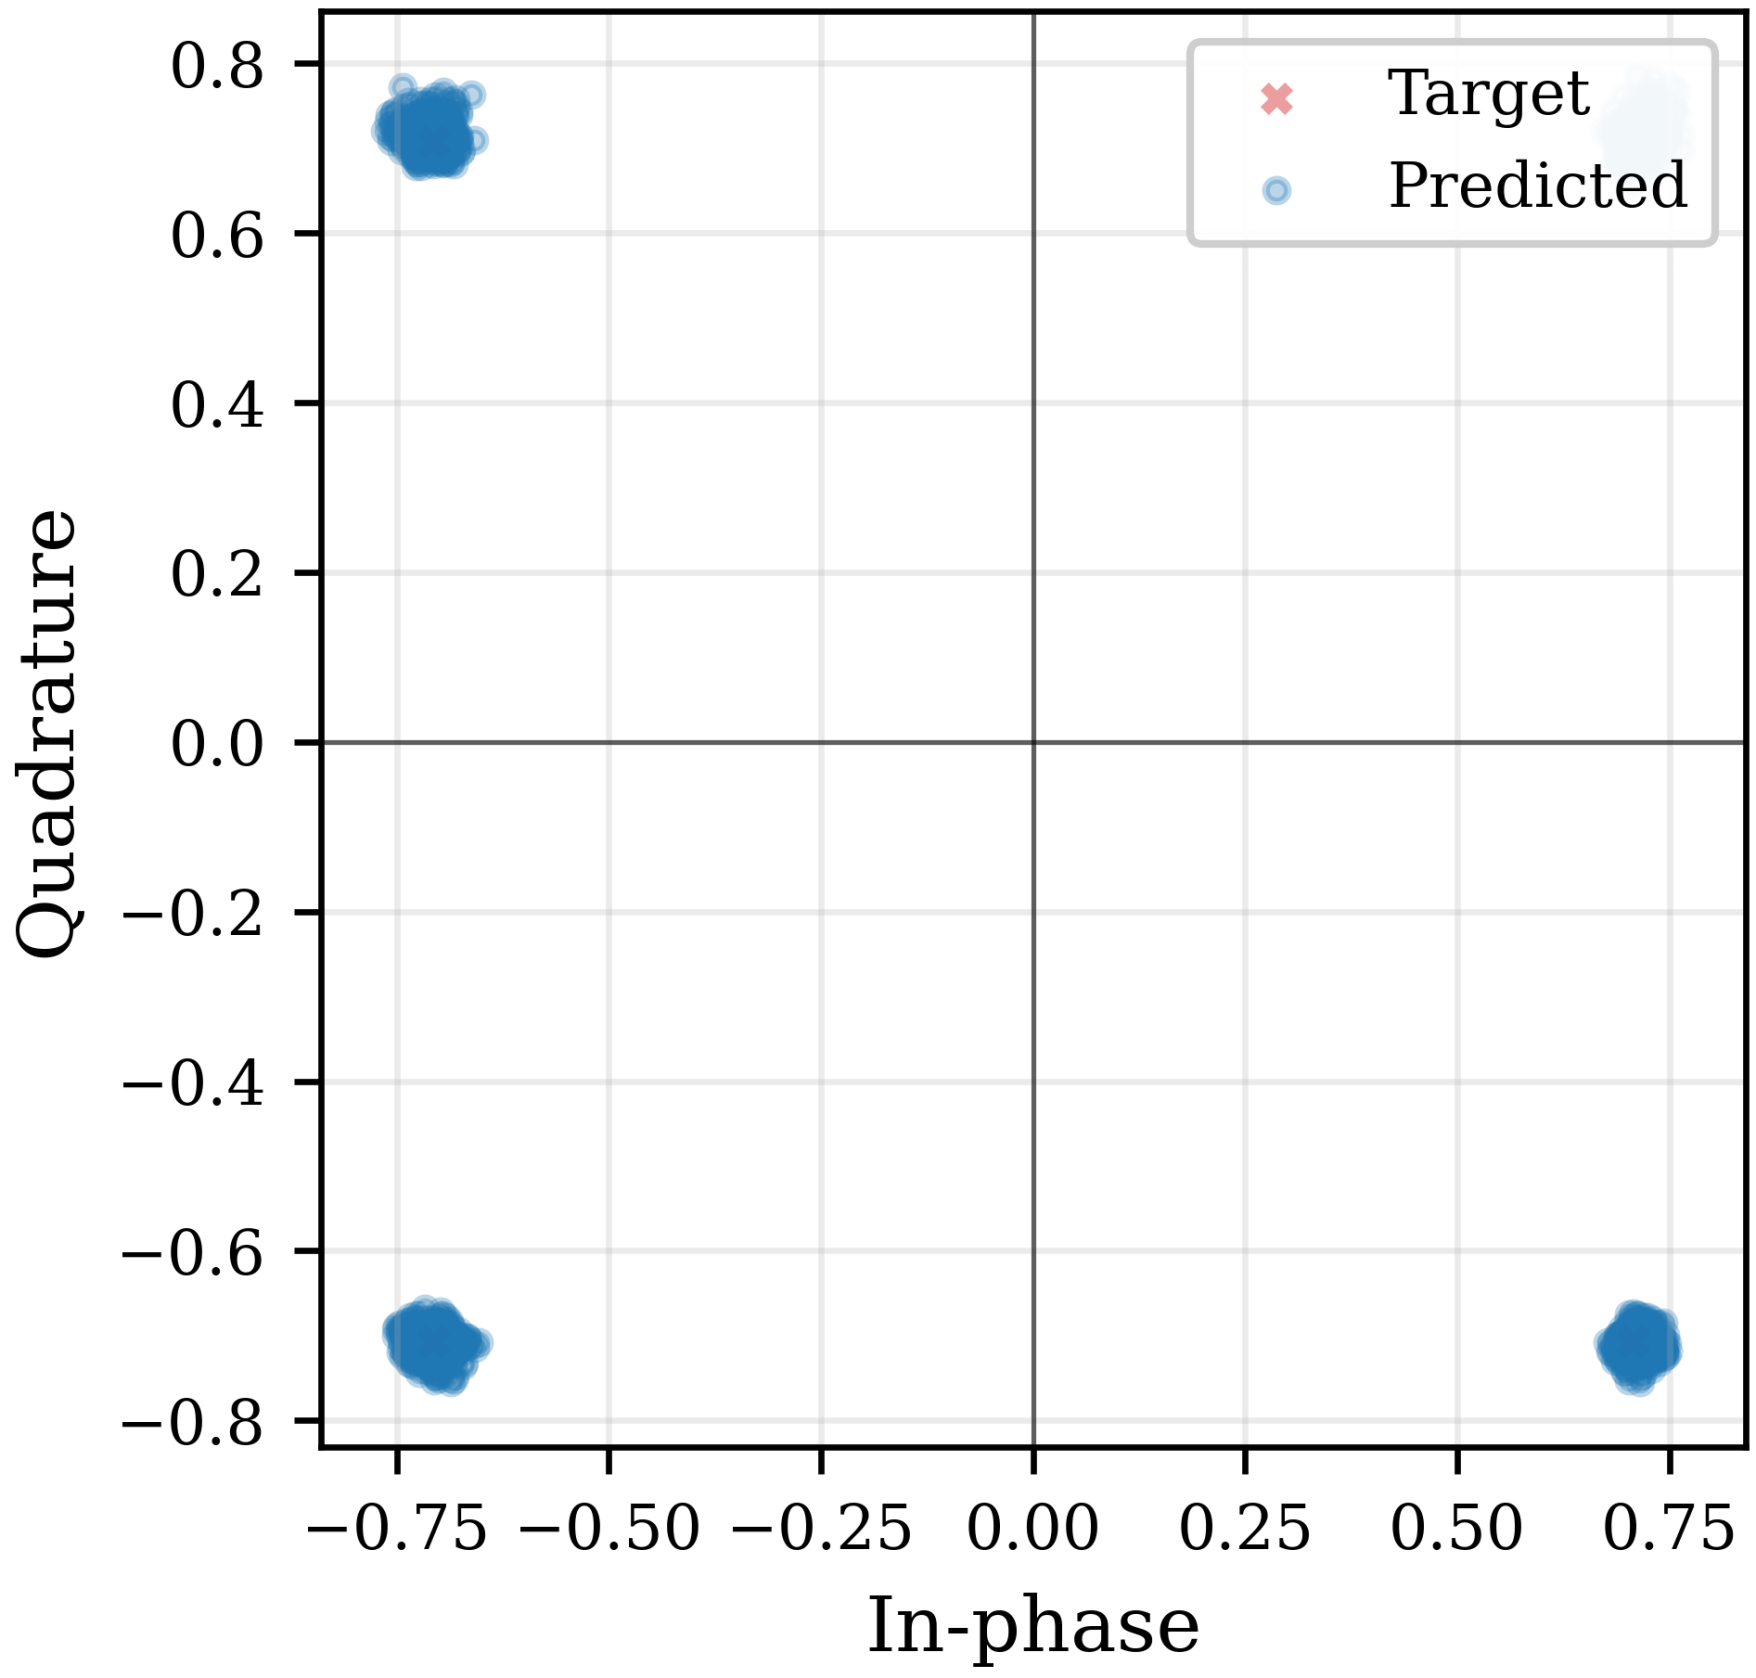
\includegraphics[width=\subfigw]{images/neural/results/cnn_constellation_convnext_tiny_curriculum_lvl2_weak.png}%
} &
\subfloat[Moderate.\label{fig:neural_const_moderate}]{%
  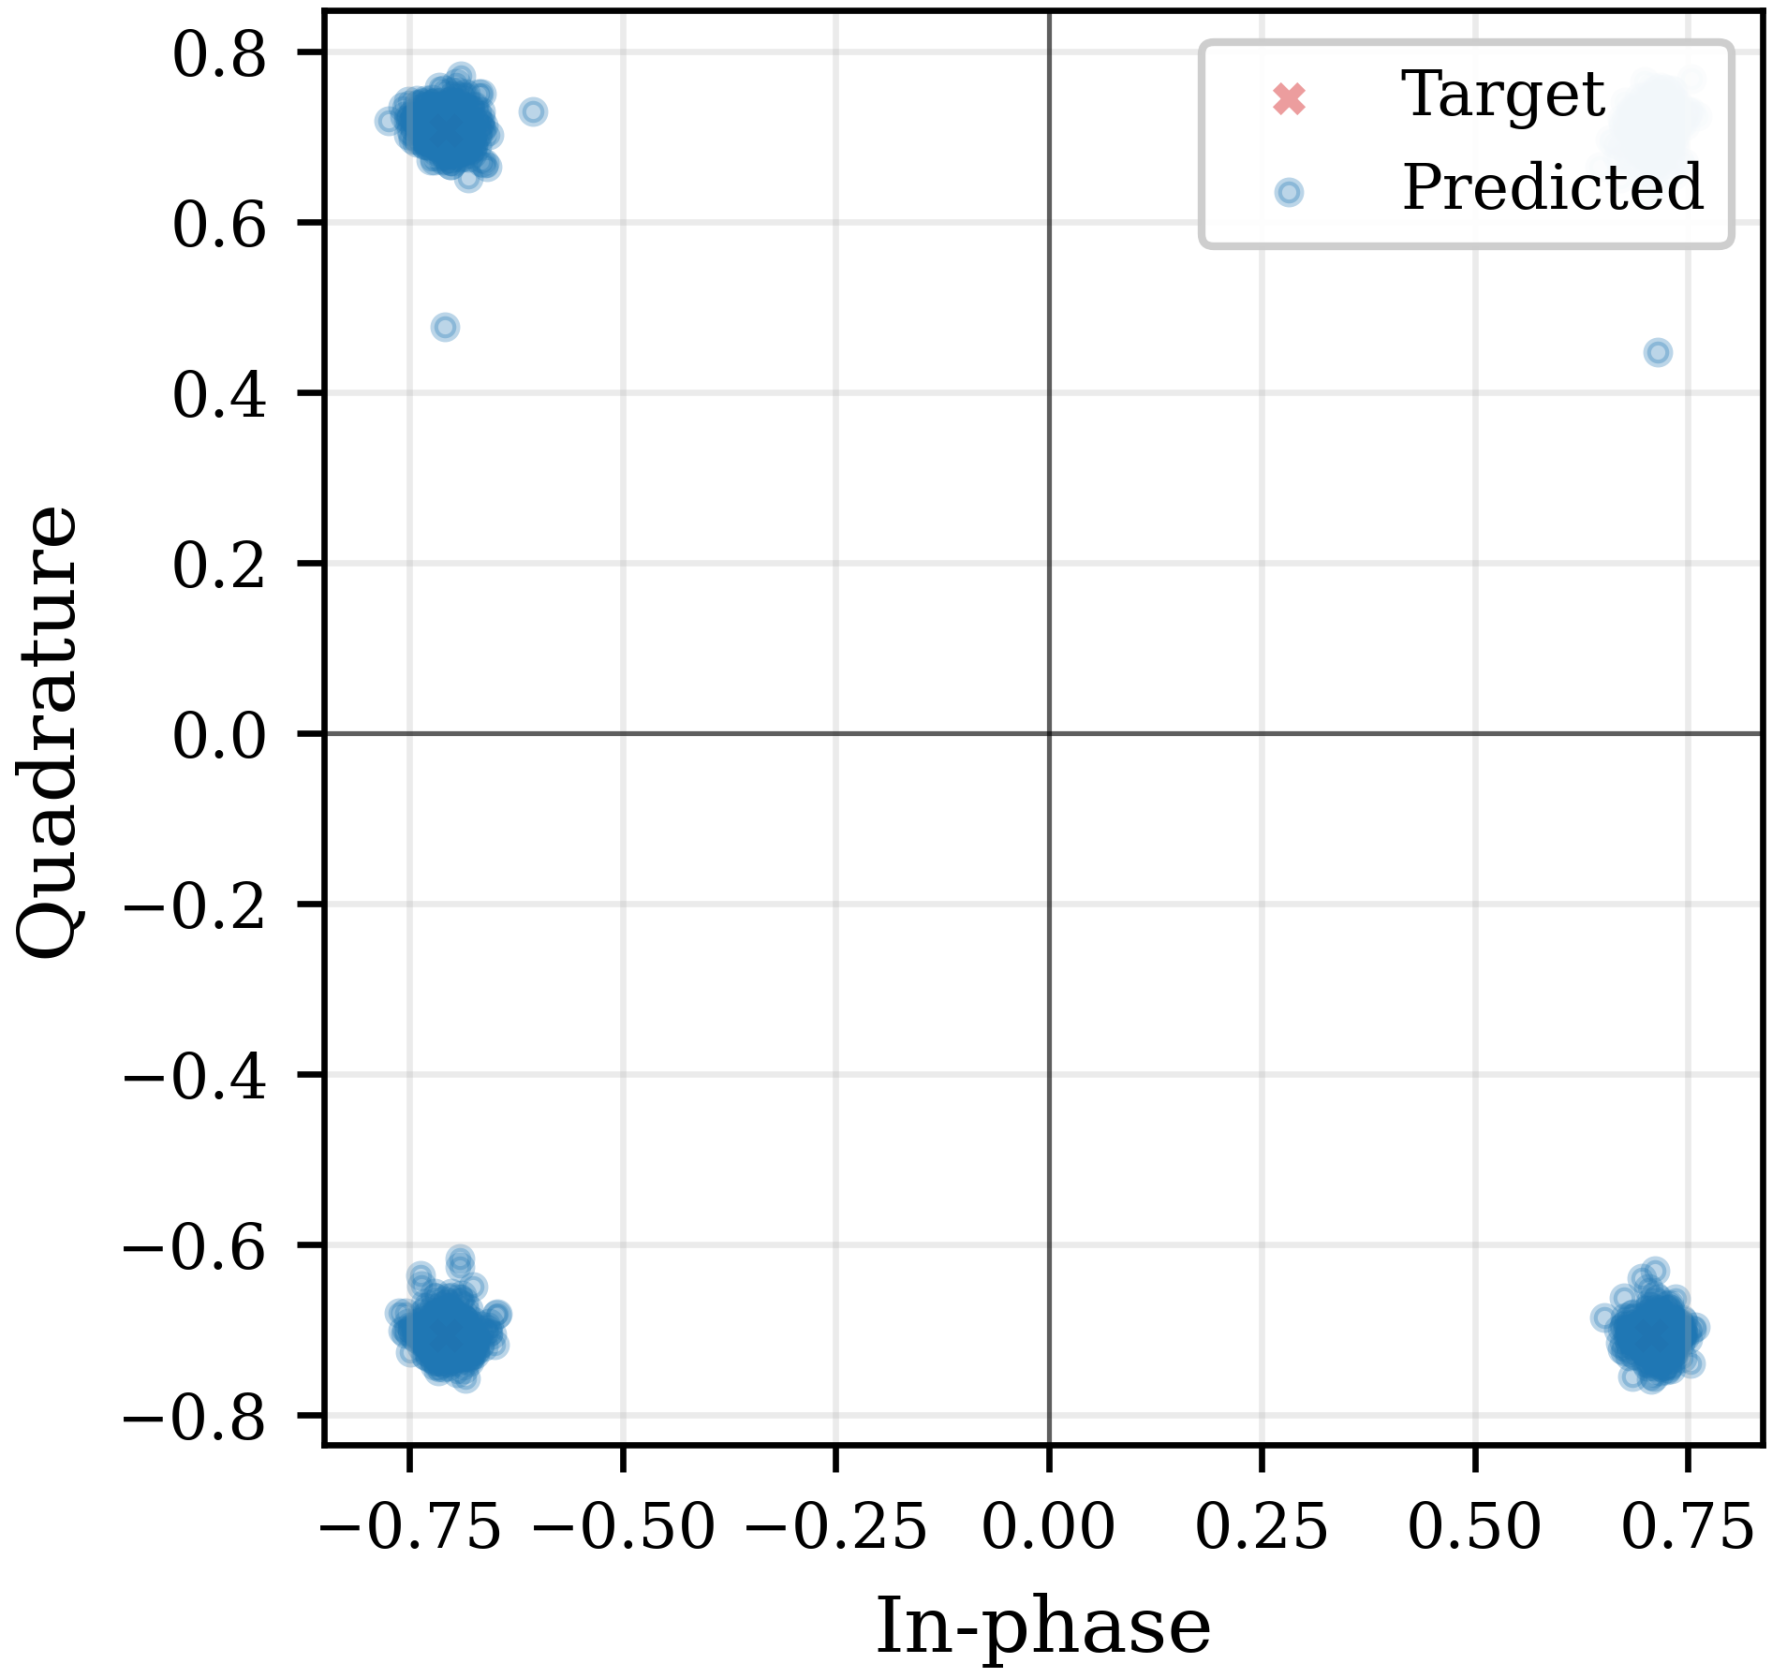
\includegraphics[width=\subfigw]{images/neural/results/cnn_constellation_convnext_tiny_curriculum_lvl3_moderate.png}%
}
\end{tabular}\\[0.8ex]
\makebox[\textwidth][c]{%
\begin{tabular}{@{}c@{\hspace{\subfiggap}}c@{}}
\subfloat[Strong.\label{fig:neural_const_strong}]{%
  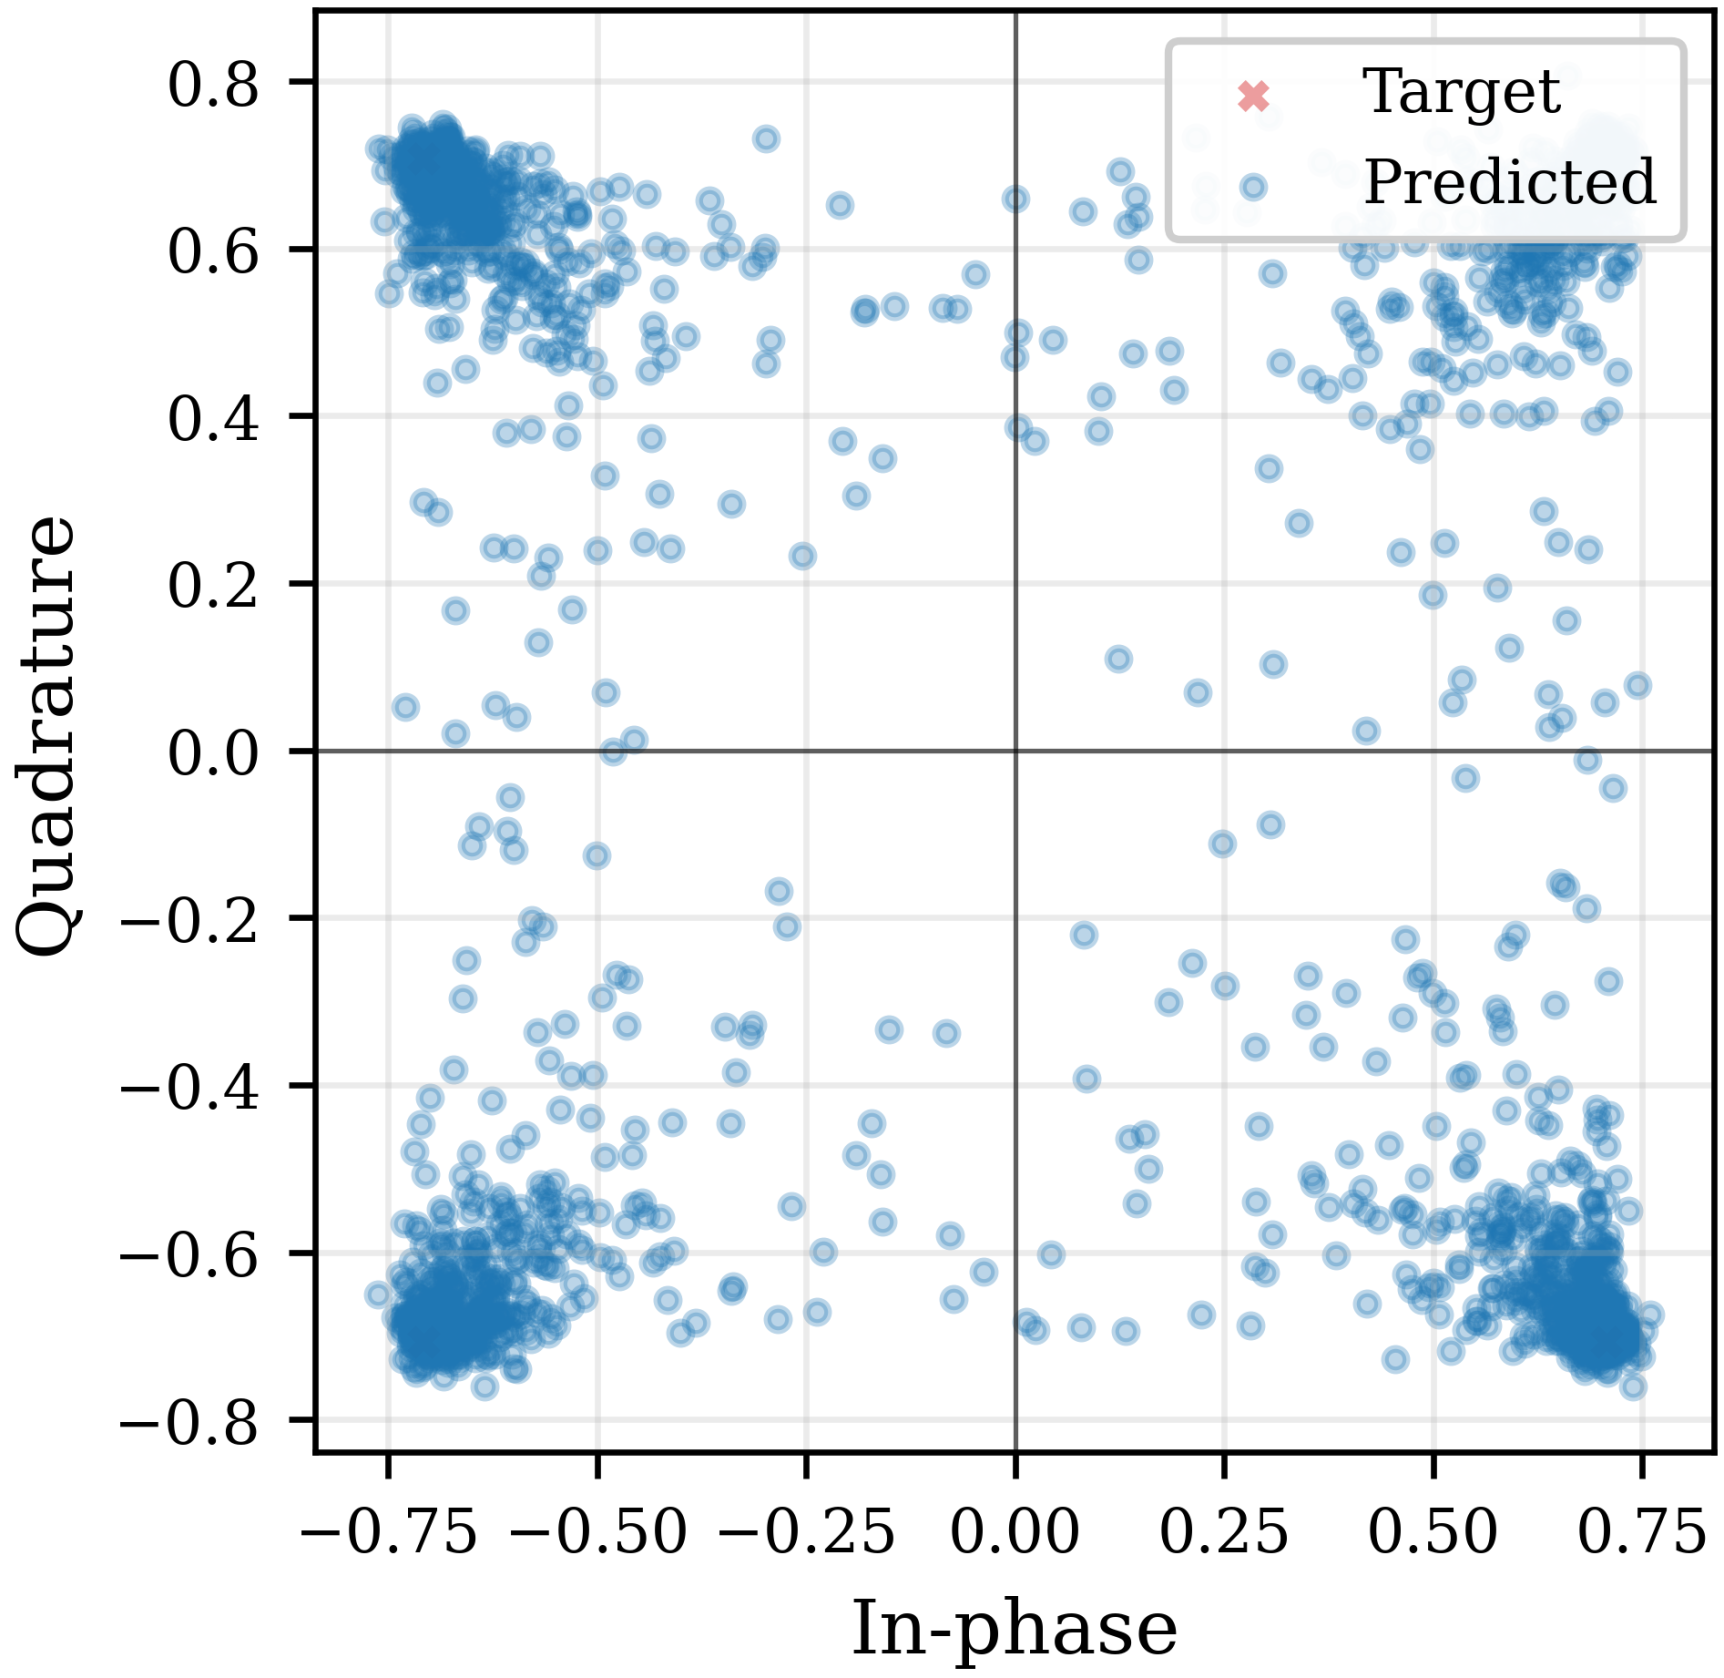
\includegraphics[width=\subfigw]{images/neural/results/cnn_constellation_convnext_tiny_curriculum_lvl4_strong.png}%
} &
\subfloat[Extreme.\label{fig:neural_const_extreme}]{%
  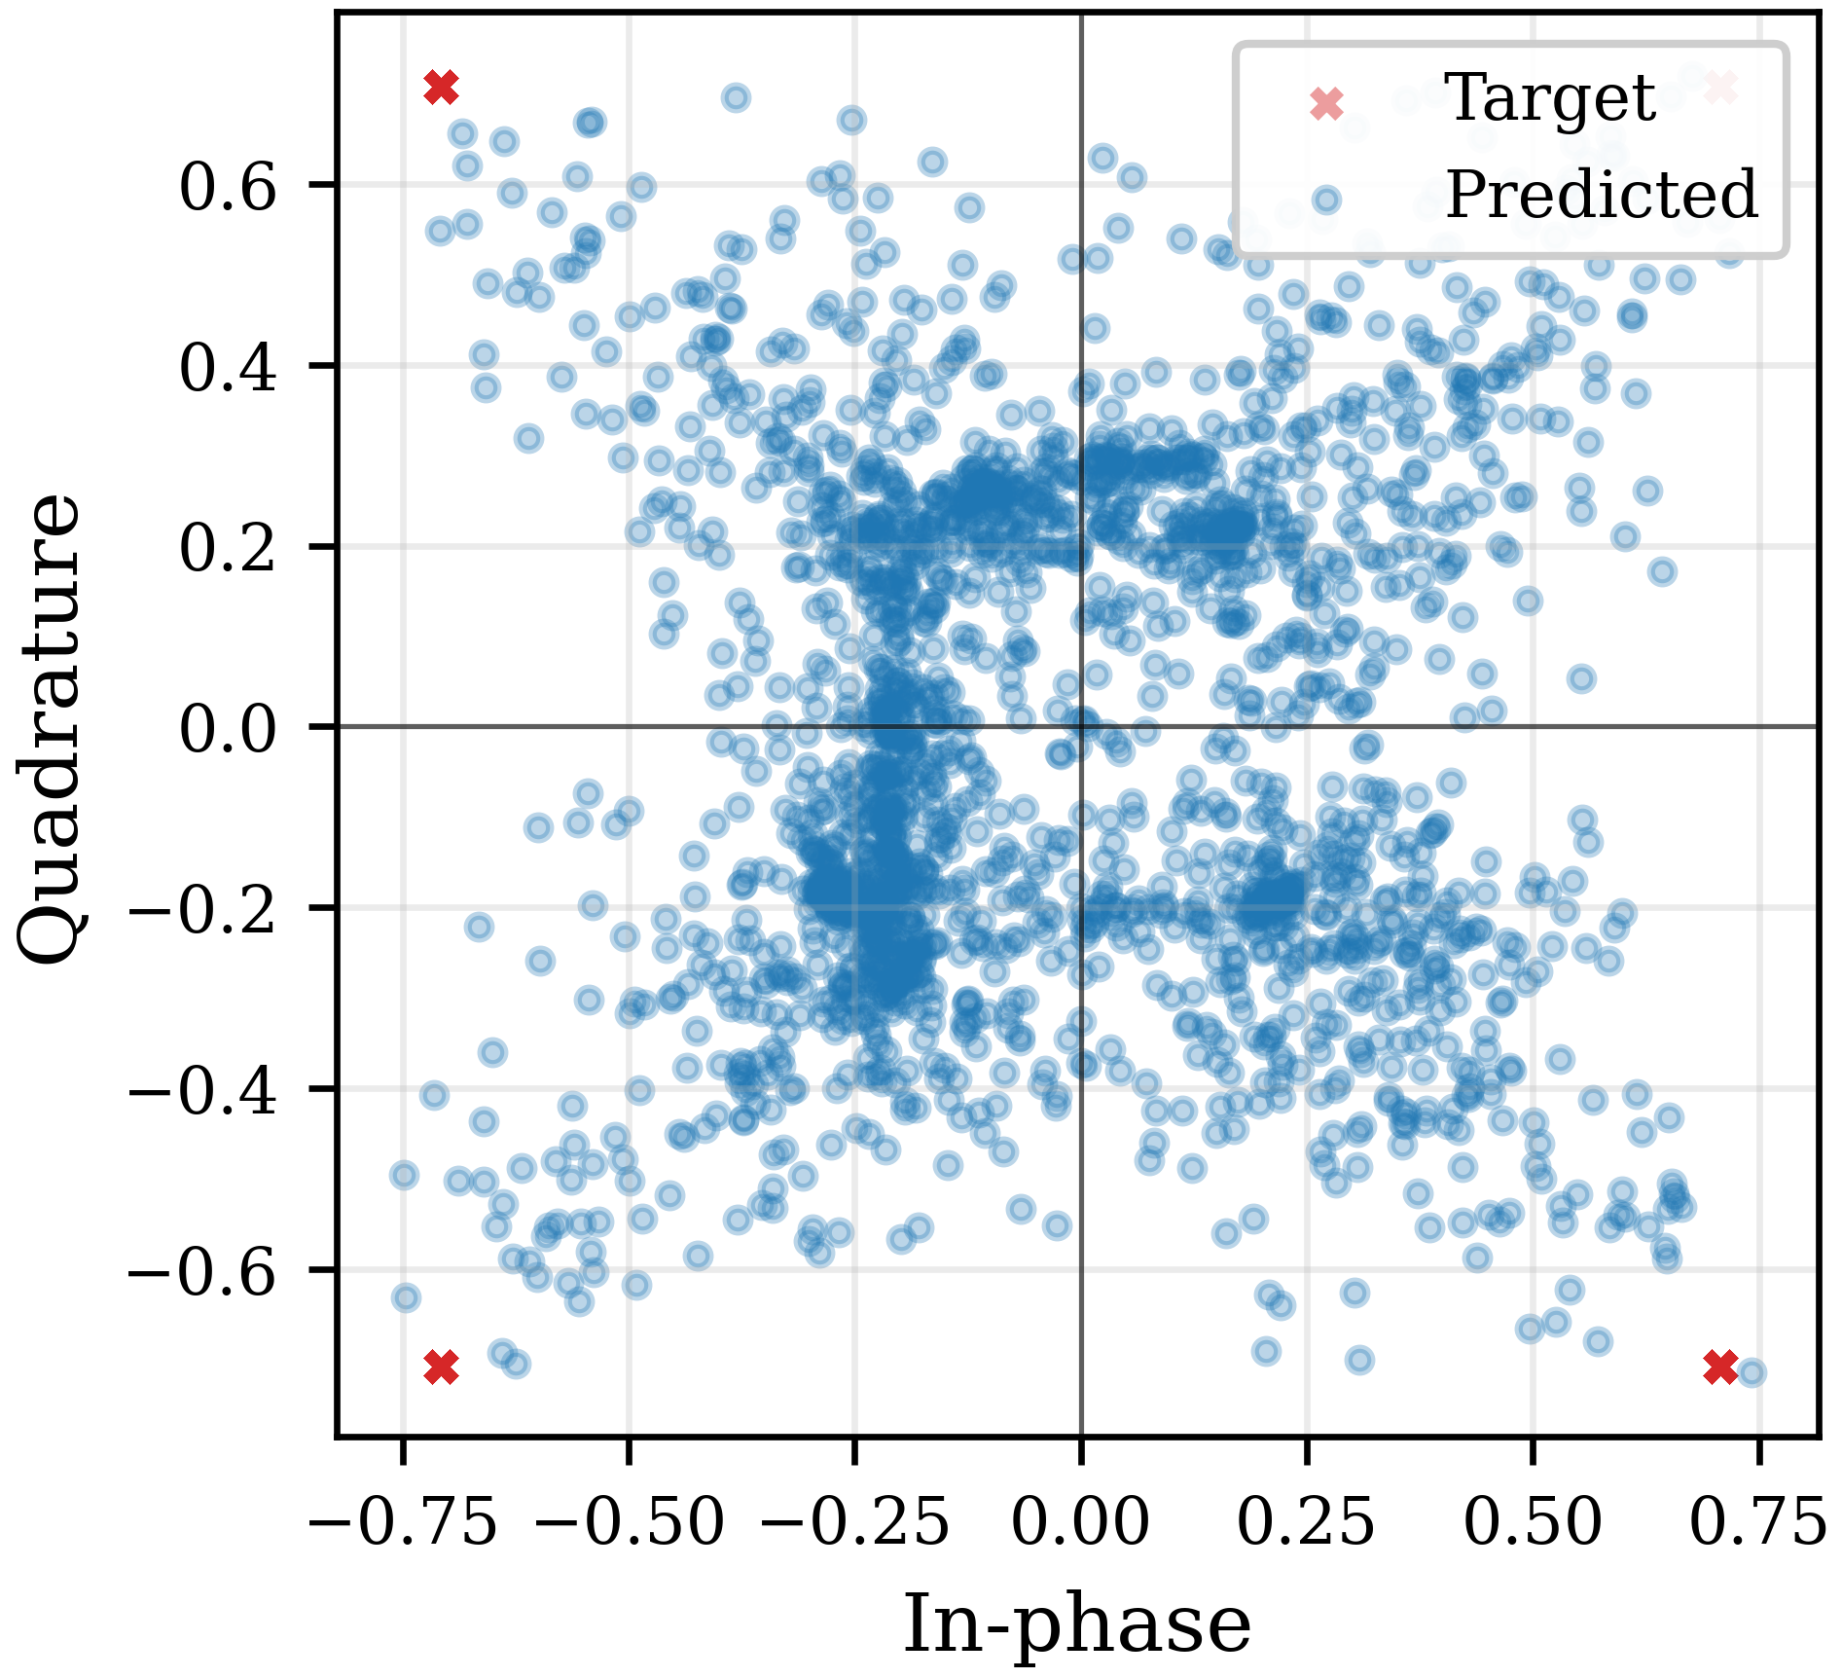
\includegraphics[width=0.33\textwidth]{images/neural/results/cnn_constellation_convnext_tiny_curriculum_lvl5_extreme.png}%
}
\end{tabular}
}
\caption{Neural-receiver constellations at each curriculum stage. Clear four-way clusters in the ideal and weak cases give way to widening scatter in the strong regime; by the extreme stage the original decision boundaries are largely gone.}
\label{fig:neural_stage_constellation_progression}
\end{figure*}

Through the ideal stage, the neural receiver essentially hits the measurement floor (around $10^{-5}$) and stays there; the weak stage is similar, with only the occasional isolated excursion. The moderate stage is more mixed: lower $C_n^2$ values are still near the floor, but several bins climb into the $10^{-3}$--$10^{-2}$ range as turbulence approaches $10^{-15}$. The degradation appears gradual rather than abrupt, which suggests the learned mapping does not break down all at once as distortion strengthens.

The strong and extreme stages are where things get noticeably worse. In the strong interval ($10^{-15}$--$10^{-14}$), BER climbs well above the floor and tends to sit somewhere between $10^{-2}$ and a few times $10^{-1}$, reaching around $0.28$ near the top of the range. In the extreme interval ($10^{-14}$--$10^{-12}$), BER opens near $0.3$ and climbs toward $0.5$, which in practice means the model is making nearly random decisions for much of that range. This is visible in the constellation plots too: clean four-way QPSK clusters in the ideal case gradually broaden and eventually collapse into a diffuse central cloud in the extreme stage, where the original decision boundaries are largely gone.

Relative to the classical chain, the neural receiver holds up best in the weak and lower-moderate range, roughly where the classical chain starts to climb because of ill-conditioning. The neural model also degrades under strong turbulence, but the combined view suggests the drop to near-random performance is delayed until the extreme stage rather than occurring right at transition. Overall, this indicates a limited but real role for intensity-only recovery in moderate turbulence, where coherent inversion is already under stress. It should not be expected to remain effective under the strongest distortions, consistent with prior reports of turbulence-driven OAM mode mixing and phase sensitivity~\cite{paterson2005atmospheric, ren2013atmospheric}.

\begin{table}[htbp]
\centering
\caption{Qualitative Summary of Classical Baseline Behavior}
\label{tab:performance_summary}
\small
\renewcommand{\arraystretch}{1.12}
\begin{tabularx}{\columnwidth}{l l X}
\toprule
\textbf{Regime} & \textbf{$C_n^2$ Range} & \textbf{Baseline Behavior} \\
\midrule
Weak & $\lesssim 10^{-16}$ & Modal orthogonality preserved; BER $<10^{-2}$; $\kappa(\hat{\mathbf{H}}) \approx 1$. \\
Transition & $10^{-15}$--$10^{-14}$ & Crosstalk rises; BER increases from $\approx$0.01 to $\approx$0.5; coding gain collapses; $\kappa(\hat{\mathbf{H}}) \approx 3$--$17$. \\
Strong/Extreme & $\gtrsim 10^{-14}$ & Channel mixing dominates; BER $\approx$ 0.5; $\kappa(\hat{\mathbf{H}}) \gtrsim 17$. \\
\bottomrule
\end{tabularx}
\end{table}


% \FloatBarrier

The classical MMSE chain requires a matrix inversion every symbol slot ($O(M^3)$, manageable for $M=8$), whereas the neural receiver pays its main cost during training and then runs at fixed latency once deployed.

% \FloatBarrier
%==============================================================================
% V. CONCLUSION
%==============================================================================
\section{Conclusion}
\label{sec:conclusion}

From a wireless-system perspective, the results separate three operational regimes for the considered OAM link: a weak-turbulence regime where pilot-aided coherent processing and FEC remain effective, a transition where $\kappa(\hat{\mathbf{H}})$ rises and soft information quality collapses, and a strong regime where reliable decoding is not supported by either the classical or intensity-only architectures tested here. The numerical framework itself is the enabling artifact: one propagation model, one $C_n^2$ sweep, and two receiver classes that differ only in observation and algorithm, which is the comparison pattern TWC readers expect when judging new receiver ideas against a verifiable reference.

Design implications are as follows. First, any learning-based OAM receiver should be reported against a full channel-estimation and FEC chain under matched statistics, not in isolation or on mismatched physics. Second, intensity-only CNNs can narrow the implementation gap where coherent optics are unavailable, but in our experiments they do not fully recover the performance lost when phase information is unavailable at the receiver; their utility in moderate turbulence should be weighed against hardware and latency costs of coherent reception. Third, Table~\ref{tab:ber_key} underscores that a single BER point is insufficient---$\kappa(\hat{\mathbf{H}})$ and pre/post-FEC curves together explain \emph{why} performance changes.

Limitations include simulation-only validation, a single range and geometry, two channel realizations per $C_n^2$ in Section~\ref{sec:results}, and a neural path without LDPC so that comparisons stay at a consistent symbol metric. Outdoor links would add temporal fading, misalignment, and aperture effects beyond Kolmogorov screens alone~\cite{andrews2005laser}.

Future work may (i)~fuse intensity features with partial coherent measurements or sparse pilots, (ii)~train neural decoders that consume LLRs jointly with classical front ends, (iii)~scale $M$ and distance, and (iv)~field-test regimes where the simulator predicts usable performance. These directions extend the baseline established here rather than replacing it.

% \FloatBarrier
\bibliographystyle{IEEEtran}
\bibliography{references}

\end{document}


